%%%%%%%%%%%%%%%%%%%%%%%%%%%%%%%%%%%%%%%%%%%%%%%%%%
% MS TODO's
%
% * find/replace "centrifugally supported" with something less
% jargony, and more physically meaningful.  (read CR89)
%
% * "Bound-free absorption can provide
%   wavelength-dependent opacity, but the absorption coefficients
%   generally {\it grow} with increasing wavelength, rather than {\it
%   shrink} as one needs in order to get deeper absorption in the blue
%   than in the red."
%   --> Isn't this statement wavelength dependent????
%
%
%%%%%%%%%%%%%%%%%%%%%%%%%%%%%%%%%%%%%%%%%%%%%%%%%%

% upon AAS submission
%\documentclass[12pt,twocolumn,tighten,linenumbers]{aastex63}
%\documentclass[12pt,twocolumn,tighten,linenumbers,trackchanges]{aastex63}
% drafting / arxiv
\documentclass[11pt,twocolumn,tighten]{aastex63}
\turnoffedit

\usepackage{apjfonts}
\usepackage{url}
\usepackage{hyperref}
\usepackage{natbib}
\usepackage{amsmath,amstext,amssymb}
\usepackage[caption=false]{subfig} % for subfloat
\usepackage{xcolor, fontawesome}
\usepackage{color}
\usepackage{enumitem}

\newcommand{\rprs}{{$R_p/R_{\star}$}}
\newcommand{\vsini}{{$V \sin i$}}
\newcommand{\kms}{{km\,s$^{-1}$}}
\newcommand{\gcc}{{g\,cm$^{-3}$}}
\newcommand{\rstar}{{$R_\star$}}
\newcommand{\rhostar}{{$\rho_\star$}}
\newcommand{\mearth}{{M$_\oplus$}}
\newcommand{\rearth}{{R$_\oplus$}}
\newcommand{\rsun}{{$R_\odot$}}
\newcommand{\msun}{{$M_\odot$}}
\newcommand{\bprp}{G_{\rm BP} - G_{\rm RP}}

\newcommand{\minus}{\scalebox{0.5}[1.0]{$-$}}

\newcommand{\mstype}{letter}

%%%%%%%%%%%%%%%%
% INSTITUTIONS %
%%%%%%%%%%%%%%%%
\newcommand{\caltech}{Department of Astronomy, MC 249-17, California Institute of Technology, Pasadena, CA 91125, USA}
\newcommand{\mitkavli}{MIT Kavli Institute and Department of Physics, 77 Massachusetts Avenue, Cambridge, MA 02139}
\newcommand{\berkeley}{Astronomy Department, University of California, Berkeley, CA 94720, USA}
\newcommand{\princeton}{Department of Astrophysical Sciences, Princeton University, 4 Ivy Lane, Princeton, NJ 08540, USA}
\newcommand{\esa}{European Space Agency (ESA), European Space Research and Technology Centre (ESTEC), Keplerlaan 1, 2201 AZ Noordwijk, Netherlands}

%
% ms specific numbers
%

%%%%%%%%%
% STARS %
%%%%%%%%%
\newcommand{\nstarssearched}{65760}
\newcommand{\nlcssearched}{180017}


%%%%%%%%
% CQVS %
%%%%%%%%

% dip-counting pipeline
\newcommand{\nuniqdipflagged}{{368}} % up-to-date; get_lgb_list_count.py

\newcommand{\ncpvsfound}{70}
\newcommand{\ngoods}{53}
\newcommand{\nmaybes}{17}
\newcommand{\ngoodsfieldbanyan}{three}
\newcommand{\nmaybesfieldbanyan}{0}
\newcommand{\ngoodsnotfieldbanyan}{52}
\newcommand{\nmaybesnotfieldbanyan}{17}
\newcommand{\nnotfieldbanyan}{69}


\begin{document}

%\title{Pre-Main-Sequence M-Dwarfs With Complex Quasiperiodic Variability From Four Years of TESS}
%\title{Complex Quasiperiodic Variables From Four Years of TESS}
\title{Corotating Clumps Around Adolescent Low-Mass Stars: Four Years of TESS}

\correspondingauthor{Luke G. Bouma}
\email{luke@astro.caltech.edu}

\received{---}
\revised{---}
\accepted{---}
\shorttitle{Four Years of CQVs} 

\shortauthors{Bouma, Jayararaman, et al.}

%%%%%%%%%%%%%%%%%%%%%%%%%%%%%%%%%%%%%%%%%%
%%%%%%%%%%%%%%%%%%%%%%%%%%%%%%%%%%%%%%%%%%
%%%%%%%%%%%%%%%%%%%%%%%%%%%%%%%%%%%%%%%%%%

% primary authors
\author{---AUTHOR LIST \& ORDER NOT FINAL}
\author[0000-0002-0514-5538]{Luke~G.~Bouma}
\altaffiliation{51 Pegasi b Fellow}
\affiliation{\caltech}

\author[0000-0002-7778-3117]{Rahul~Jayararaman}
\affiliation{\mitkavli}

\author{Lynne~A.~Hillenbrand}
\affiliation{\caltech}

\author[0000-0001-7204-6727]{G\'asp\'ar \'A. Bakos}
\affiliation{\princeton}

\author{-----SUGGESTED CONTRIBUTORS, PENDING DISCUSSION, COMMENTS, ANALYSES, ETC-----}
%
\author{Saul~Rappaport}
\affiliation{\mitkavli}

\author[0000-0001-6381-515X]{Luisa M. Rebull}
\affiliation{\caltech}

\author[0000-0002-3164-9086]{Maximilian N. G\"unther}
\affiliation{\esa}

\author[0000-0003-2058-6662]{George~R.~Ricker}
\affiliation{\mitkavli}

\author[0000-0002-4265-047X]{Joshua N. Winn}
\affiliation{\princeton}


%%%%%%%%%%%%%%%%%%%%%%%%%%%%%%%%%%%%%%%%%%
%%%%%%%%%%%%%%%%%%%%%%%%%%%%%%%%%%%%%%%%%%
%%%%%%%%%%%%%%%%%%%%%%%%%%%%%%%%%%%%%%%%%%

% 250 word max!
\begin{abstract}
  Complex quasiperiodic variables (CQVs) are low-mass
  pre-main-sequence stars with nearly periodic optical modulation.
  The modulation is likely induced by dust or gas clumps in orbit at
  the Keplerian corotation radius.  Here, we report new CQVs
  discovered in TESS short-cadence data collected between July~2018
  and Sep~2022.  Our search of \nstarssearched\ K- and M-dwarfs with
  $T$$<$16 and $d$$<$150\,pc yielded \ngoods\ high-quality CQVs.  Most
  of these discoveries are new, and they include the brightest
  ($T$$\approx$9.5) and closest ($d$$\approx$20\,pc) examples of this
  class of object known, and probably also the most massive
  ($\approx$0.6-0.8\,$M_\odot$) and oldest ($\approx$200\,Myr).  A few
  objects are outliers among outliers; LP 12-502 for instance shows a
  recurring ``dip complex'' with a period and total duration that are
  fixed over more than 1{,}000 cycles, but which in detail exhibits
  anywhere from four to eight local minima per cycle.  LP 12-502 also
  displayed distinct superposed periods simultaneously, and showed
  drastic shape changes shortly after flares.  Broadly speaking, we
  find that none of the CQVs maintain a fixed light curve shape over
  timescales of more than a few hundred cycles, and we revisit the
  arguments for why transient corotating material is the most viable
  explanation.  In the future, we expect that our sample will
  facilitate modeling and observational efforts aimed at understanding
  these objects, and connecting them to the broader contexts of star,
  disk, and exoplanet evolution.  For instance, if the transiting
  material is dust, then the rate of dip evolution implies that of
  order an asteroid belt's worth of mass passes through these
  structures over their lifetime of $\approx$$10^8$ years.
\end{abstract}


\keywords{Weak-line T Tauri stars (1795),
Periodic variable stars (1213),
Circumstellar matter (241),
Star clusters (1567),
Stellar magnetic fields (1610),
Stellar rotation (1629)}


\section{Introduction}
\label{sec:intro}

All pre-main-sequence stars vary in optical brightness, and the origin
of such variability is, in most cases, understood.  Well-explored
sources of optical variability include inhomogeneities on stellar
surfaces such as starspots and faculae \citep{2021isma.book.....B},
occultations by gas-rich circumstellar disks
\citep{2017MNRAS.470..202B}, and, in geometrically favorable
circumstances, eclipses by stars and planets
\citep{2010exop.book...55W}.  More exotic forms of optical variability
relevant to this work include transiting exocomets (e.g.~$\beta$~Pic;
\citealt{2019A&A...625L..13Z}) and disintegrating rocky bodies around
both M-dwarfs (e.g. KOI-2700; \citealt{2014ApJ...784...40R}) and white
dwarfs (e.g. WD~1145; \citealt{2015Natur.526..546V}).

Data from K2 and TESS have yielded a new class of variable star whose
root cause is only beginning to become clear: complex quasiperiodic
variables (CQVs).  These objects are identified phenomenologically
using their optical light curves, which show nearly periodic troughs
that can be either sharp or broad, often superposed on smooth
spot-like modulation
\citep{2017AJ....153..152S,2018AJ....155...63S,2019ApJ...876..127Z}.
Some CQVs show up to eight local minima (dips) per cycle.  Most are
pre-main-sequence M-dwarfs without near-infrared excesses, ages of
$\approx$5-150 million years (Myr), and rotation periods of at most
two days; they are observed to be $\approx$1-3\% of M-dwarfs younger
than 100 Myr \citep{2016AJ....152..114R,2022AJ....163..144G}.  The
dips can be chromatic, with a reddening law plausibly consistent with
dust
\citep{2020AJ....160...86B,2022AJ....163..144G,2023MNRAS.518.2921K}.
And finally, while the dip shapes can ``jump'' between different
depths and durations over less than one cycle, they more often evolve
gradually, over tens to hundreds of cycles
\citep[e.g.][]{2017AJ....153..152S,2022ApJ...925...75P,2023ApJ...945..114P}.

A few competing explanations for what causes the complex quasiperiodic
variability are shown in Figure~\ref{fig:f1}.  All young M-dwarfs are
spotted, which produces flux variations over characteristic timescales
of the rotation period, $P_{\rm rot}$, and its half-harmonic,
$0.5\,P_{\rm rot}$.  The observed dips occur over durations as short
as $0.05\,P_{\rm rot}$; a ``starspot-only'' scenario can be discarded
for any object with sufficiently sharp dips
\citep{2017AJ....153..152S,2021MNRAS.500.1366K}.   The timescales and
amplitudes of the flux variations instead require sharp geometries
with material extrinsic to the stellar surface
\citep[e.g.][]{2017AJ....153..152S,2022AJ....163..144G}.  The
``clump'' scenario invokes opaque dust clumps orbiting near the
Keplerian corotation radius, which periodically eclipse the star
\citep{2017AJ....153..152S,2023MNRAS.518.4734S}.  The ``prominence''
scenario invokes long-lived condensations of cool and dense
marginally-ionized gas, embedded within the hotter corona, that would
be centrifugally supported near corotation
\citep{1989MNRAS.238..657C,2019MNRAS.482.2853J,2022MNRAS.514.5465W}.
Such structures are analogous to quiescent prominences and filaments
seen in the solar corona \citep[see e.g.][]{2015ASSL..415.....V},
though at much larger relative distances from the stellar surface.  A
final possibility that has been suggested is one of a ``screen'', in
which the inner wall of a quiescent circumstellar disk blocks a
portion of the stellar surface to produce sudden dips whenever spots
come into view \citep{2019ApJ...876..127Z}.  

The dust clump and prominence hypotheses seem most plausible.  They
are qualitatively similar, except that one invokes opacity from dust,
while the other invokes opacity from gas, likely bound-free
transitions in hydrogen or perhaps a molecular opacity.  The screen
scenario seems inconsistent with the degree of observed periodicity,
the lack of infrared excess, and the observed lifetime of CQVs
extending an order of magnitude longer than the $\approx$$10^7$ year
timescale typically quoted for primordial disk dispersal.  However,
unambiguous evidence in support of any one scenario has yet to be
acquired.  Such evidence might include a spectroscopic detection of
silicate 10\,$\mu$m dust absorption during a dip, or perhaps detection
of transient Balmer-line absorption as a function of cycle phase,
similar to observations made in systems such as AB~Dor \citep[see the
review by][]{1999ASPC..158..146C}.

CQVs remain mysterious because they have been both hard to discover
and hard to characterize.   Discoverability is tied to rarity: CQVs
comprise $\approx$1\% of the youngest $\approx$1\% of M-dwarfs
\citep{2018AJ....155..196R}.  Out of the millions of stars monitored
by K2 and TESS, about 50 CQVs have been reported to date
\citep{2016AJ....152..114R,2017AJ....153..152S,2018AJ....155...63S,2019ApJ...876..127Z,2020AJ....160...86B,2022AJ....163..144G,2023ApJ...945..114P}.
The known CQVs are correspondingly faint; the initial K2 discoveries
\citep{2016AJ....152..114R,2017AJ....153..152S} were M2-M6 dwarfs at
distances $\gtrsim$100\,pc, yielding optical brightnesses of
$V$$\approx$15.5 to $V$$>$20.  This renders time-series spectroscopy
at high resolution out of reach for current facilities, despite its
potential utility in ruling between the models.

In this work, we aim to find bright and nearby CQVs, since these
objects will be the most amenable to detailed photometric and
spectroscopic analyses.  To do this, we use 120-second cadence data
acquired by TESS between July~2018 and Sep~2022 (Sectors 1-55; Cycles
1-4).  We present our search methods in Section~\ref{sec:methods}, and
the properties of the resulting CQV catalog in
Section~\ref{sec:results}.  The evolution of many CQVs over a two-year
baseline is described in Section~\ref{sec:evoln}, including a
deep-dive into LP 12-502.  We describe a few implications in
Section~\ref{sec:discussion}, and conclude in
Section~\ref{sec:conclusion}.

A point on nomenclature.  CQVs have been called ``transient flux
dips'', ``persistent flux dips'', ``scallop shells'', ``batwings'',
\citep{2017AJ....153..152S} ``complex rotators'',
\citep{2019ApJ...876..127Z,2022AJ....163..144G,2023ApJ...945..114P}
and ``complex periodic variables'' \citep{2023MNRAS.518.2921K}.  The
CQVs should not be conflated with ``dippers'', which are classical T
Tauri stars with infrared excesses, and large-amplitude variability
linked to obscuring inner disk structures and accretion hot spots
\citep{2014AJ....147...82C,2021ApJ...908...16R}.  With that said, a
few similarities between CQVs and dippers do exist (see
Sections~\ref{subsec:irexcess} and~\ref{subsec:discdippers}).  At the
risk of introducing yet another standard, we hope to introduce a
nomenclature that reflects how, when observed over timescales of more
than tens of cycles, CQVs are almost but not exactly periodic.  They
are quasiperiodic.  While the three-type classification scheme
proposed by \citet{2017AJ....153..152S} may indeed provide some
helpful visual distinctions amongst the CQVs, it seems likely that
they are all explained by a single underlying phenomenon, and so we
opt to refer to them by a single empirically descriptive name.


\begin{figure*}[!t]
	\begin{center}
		\subfloat{
			\includegraphics[width=0.8\textwidth]{f1a.pdf}
		}
		
		\vspace{-0.6cm}
		\subfloat{
			\includegraphics[width=0.8\textwidth]{f1b.pdf}
		}
	\end{center}
		\vspace{-0.3cm}
	\caption{
		{\bf Complex quasiperiodic variables (CQVs)}:
    {\it Top:} Phase-folded TESS light curves of three CQVs.  Each is
    stacked over one month.  Gray circles are raw 2-minute data; black
    circles bin to 300 points per cycle.  Periods in hours are in the
    bottom right of each panel.  Left-to-right, the objects are LP
    12-502 (TIC 402980664; Sector~19), TIC 94088626 (Sector 10), and
    TIC 425933644 (Sector~28).
    {\it Bottom:} Cartoon models for the phenomenon.  The dust clump
    scenario (lower left) and prominence scenario (lower center) both
    invoke centrifugally-supported material at the corotation radius.
    We disfavor the screen scenario (see Section~\ref{sec:intro}).
	}
	\label{fig:f1}
\end{figure*}



\section{Methods}
\label{sec:methods}

\subsection{Stellar selection function}
\label{subsec:selectionfn}

We analyzed the ``short'' 120-second cadence data acquired by TESS
between July~2018 and Sep~2022 (Sectors 1-55).  Specifically, we used
the 120-second cadence light curve products produced by the 
Science Processing and Operations Center at NASA Ames
\citep{2016SPIE.9913E..3EJ}.  While the TESS data products also
include full frame images with cadences of 200, 600, and 1800 seconds,
we limited our scope in this work for the sake of simplicity in data
handling.  In exchange, we lose in both completeness and homogeneity
of the selection function.  While TESS cumulatively observed
$\approx$90\% of the sky for at least one lunar month between
July~2018 and Sep~2022, the 120-second cadence data were acquired for
only a pre-selected set of stars over Sectors 1-26, and then a
guest-investigator driven set of stars over Sectors 27-55
\citep{2021PASP..133i5002F}.

To assess the completeness of the resulting 120-second cadence data
that is the basis of this study, we cross-matched TIC8
\citep{2018AJ....156..102S} against the Gaia DR2 point-source catalog
\citep{2018A&A...616A...1G}.  We opted for Gaia DR2 rather than DR3
because the base catalog for TIC8 was Gaia DR2, which facilitated a
one-to-one crossmatch using the Gaia source identifiers.  This
exercise showed that for $T$$<$16 M-dwarfs, the TESS 2-minute data are
roughly 50\% complete at $\approx$50\,pc.  At $<$20\,pc, $\gtrsim$80\%
of the $T$$<$16 M-dwarfs have at least one sector of short-cadence
data; at $>$100\,pc, $\lesssim$10\% of such M-dwarfs have at least one
sector of short-cadence data.  Armed with this understanding, we then
used our cross-match between Gaia DR2 and TIC8 to select our stars of
interest, which we defined as stars with 120-second cadence TESS light
curves that satisfied
\begin{align}
  T &< 16 \quad&(\mathrm{Bright\ for\ TESS})\\
  \bprp &> 1.5 \quad&(\mathrm{Red\ stars\ only}) \\
  M_{\rm G} &> 4 \quad&(\mathrm{Dwarf\ stars\ only})  \\
  d &< 150\,{\rm pc} \quad&(\mathrm{Close\ stars\ only}),
\end{align}
for $M_{\rm G} = G + 5\log(\varpi_{\rm as}) + 5$ the Gaia $G$-band
absolute magnitude, $\varpi_{\rm as}$ the parallax in units of
arcseconds, and a geometric distance $d$ defined by inverting the
parallax and ignoring any zero-point correction.  This selection
function includes dwarf stars later than spectral types of
$\approx$K6V \citep{2013ApJS..208....9P} for which TESS can acquire
1\% relative precision photometry in 1 hour of observation
\citep{2015JATIS...1a4003R}.  The target sample therefore includes
\nstarssearched\ M-dwarfs and late-K dwarfs, down to $T$$<$16 and out
to $d$$<$150\,pc.




\subsection{CQV discovery}
\label{subsec:discoverymethods}

Previous methods for finding CQVs have included visually examining
stars known to be in young clusters
\citep{2016AJ....152..114R,2017AJ....153..152S}, and automatically
flagging rapid rotators with a large number of strong Fourier
harmonics \citep{2019ApJ...876..127Z}.  The latter approach still
requires visual vetting, since ``stars with many Fourier harmonics''
is a designation that includes objects such as eclipsing binaries or
multiple stars blended into a single photometric aperture.  In this
work, we implemented a new search approach based on counting the
number of sharp local minima in phase-folded light curves, while also
using the previously tested Fourier approach.  We applied these two
search techniques independently.   


\subsubsection{Counting dips}
\label{subsec:counting}

The dip counting technique aims to count sharp local minima in
phase-folded light curves.  CQVs will preferably have at least three
such minima in order to be distinct from false positives such as
synchronized and spotted binaries (``RS CVn'' stars). 

For our dip-counting pipeline, we began with the PDC\_SAP flux for
each sector, removed non-zero quality flags, and normalized the light
curve to one by dividing out its median value.  We then flattened the
light curve using a 5-day sliding median filter, as implemented in
\texttt{wotan} \citep{2019AJ....158..143H}.  On the resulting cleaned
and flattened light curve, we ran a periodogram search, opting for the
\citet{1978ApJ...224..953S} phase dispersion minimization (PDM)
algorithm implemented in \texttt{astrobase}
\citep{2021zndo...1011188B} due to its shape agnosticism.  If a period
below 2 days was identified, we reran the periodogram at a finer grid
to improve the accuracy of the period determination.

Once a star's period $P$ was identified, we binned the phased light
curve to 100 points per cycle.  To separate ``sharp'' local minima
from smooth spot-induced variability, we then iteratively fit
penalized splines to the wrapped phase-folded light curve, excluding
points more than two standard deviations away from the local continuum
\citep{2019AJ....158..143H}.  The maximum number of equidistant spline
knots per cycle is the parameter in this framework that controlled the
meaning of ``sharp'' --- we allowed at most 10 such knots per cycle,
though for most stars fewer knots were preferred based on an
$\ell^2$-norm penalty. 

We then identified local minima in the resulting residual light curve
using the SciPy \texttt{find\_peaks} utility
\citep{2020NatMe..17..261V}, which is based on comparing adjacent
values in an array.  For a peak to be flagged as significant, we
required it to have a width of at least $0.02\,P$, and a height of at
least twice the point-to-point RMS.  This latter quantity is defined
as the 68$^{\rm th}$ percentile of the distribution of the residuals
from the median value of $\delta f_i \equiv f_i - f_{i+1}$, where $f$
is the flux and $i$ is an index over time.

To correctly identify local minima near the edges of the phased light
curve, which usually would cover phases $\phi \in [ 0,1 ]$, we 
performed the entire procedure over a phase-folded light curve
spanning $\phi \in [-1,2 ]$, by duplicating and concatenating the
ordinary phase-folded light curve.  The free parameters we adopted
throughout this analysis procedure, for instance the maximum number of
spline knots per cycle, and how large and wide of a local minimum to
consider a ``true dip'', were chosen during testing based on
their ability to correctly re-identify a large fraction ($>$90\%) of
known CQVs, while also being able to consistently reject common false
positives such as rapidly rotating spot-induced variability and
typical eclipsing binaries.

Overall, for a star to proceed to manual
examination, we required that it have a peak PDM period below two
days, and that it exhibited at least three sharp local minima (as
algorithmically reported) in at least one observed TESS sector.



\subsubsection{Fourier analysis}
\label{subsec:fourier}
For the Fourier analysis, we followed \citet{2019ApJ...876..127Z}.

{\bf TODO for Rahul or Saul: explain the approach, in a few
	paragraphs.  Was the SAP\_FLUX or PDCSAP used? etc. }

\subsubsection{Manual vetting}

\begin{figure*}[!t]
	\begin{center}
		\centering
		\includegraphics[width=0.96\textwidth]{annotated_lp12502.pdf}
		\vspace{-0.3cm}
		\caption{
			{\bf Validation plots used to  label CQVs}.  The complete figure
			set, with one image per sector for each of \ncpvsfound\ CQVs
			and CQV candidates
			is available online {\bf For internal collaboration review:
				\url{https://www.dropbox.com/scl/fo/zlj3txot4cvymfb22wewu/h?dl=0&rlkey=3ec5f9o5xewrixzfkhkdenopa}}.
			Panels are as follows.
			{\it a)}: Phase-folded light curve; gray points are raw 2-minute
			data and black points are binned to 200 points per cycle.
			{\it b)}: Phase-dispersion minimization (PDM) periodogram.
			Dotted lines show up to the 10$^{\rm th}$ harmonic and
			subharmonic.
			{\it c)}: DSS finder chart, with 1- and 2-TESS pixel radius
			circles displayed for scale.
			{\it d)}: Cleaned light curve, binned to 20-minute cadence, in
			Barycentric TESS Julian Date (BTJD).
			{\it e)}: Phase-folded light curve, binned to 100 points per
			cycle.  The gray line denotes the automated spline-fit to the
			wrapped phase-folded light curve, and small gray triangles
			denote automatically identified local minima.
			{\it f)}: Phase-folded light curve at twice the peak period.
			{\it g)}: Phase-folded light curve at half the peak period.
			{\it h)}: Phase-folded time-series within the ``background''
			aperture defined in the SPOC light curves.
			{\it i)}: Phase-folded flux-weighted centroid in the column
			direction.
			{\it j)}: Phase-folded flux-weighted centroid in the row
			direction.
			{\it k)}: Gaia DR2 color--absolute magnitude diagram.     
			The gray background denotes stars within 100\,pc.
			{\it l)}: Information from Gaia DR2, TIC8, and the automated
			dip-counting search pipeline.  ``Neighbors'', abbreviated
			``nbhr'', are listed within apparent distances of 2 TESS pixels
			if $\Delta T$$<$2.5.
			{\it m)}: BANYAN-$\Sigma$ v1.2 association probabilities, calculated
			using positions, proper motions, and the parallax.
		}
		\label{fig:vet}
	\end{center}
\end{figure*}

We visually assessed whether the objects found using the dip-counting
(Section~\ref{subsec:counting}) and Fourier
(Section~\ref{subsec:fourier}) techniques were consistent with
expectations for CQVs by assembling the data shown in
Figure~\ref{fig:vet}.  We labeled a star as a ``good'' CQV if at least
one TESS sector showed what we viewed as the unambiguous signatures of
the class (short period; at least three dips or else otherwise
oddly-shaped dips; relative stability over a timescale of 30\,days).
We independently noted stars that we thought could be CQVs, but that were more
ambiguous.

Broadly speaking, the most common false positives for both the Fourier
and dip-counting techniques were eclipsing binaries, spot-induced
variability from rapid rotators, and variability from neighboring,
off-target stars.  Typical false positive rates from our dip-counting
pipeline were 5:1, with \nuniqdipflagged\ unique stars flagged, and
about 20\% being labeled either ``good'' or ``possible'' CQVs; for
the Fourier pipeline, {\bf the rate was X:Y, with ZZZZ unique stars
flagged, and NN\% being labeled ``good'' or ``possible'' CQVs}.


\subsection{Stellar properties}
\label{subsec:starprops}

\paragraph{Ages}
We estimated the stellar ages by making probabilistic spatial and
kinematic associations between the CQVs and known clusters in the
solar neighborhood.  For most stars in our sample, we did this using
BANYAN\,$\Sigma$
\citep{2018ApJ...856...23G}.\footnote{\url{https://github.com/jgagneastro/banyan_sigma},
git commit \texttt{394b486}} This algorithm calculates the probability
that a given star belongs to one of 27 young clusters (or
``assocations'') within 150\,pc of the Sun, by modeling the clusters
as multivariate Gaussians in 3-D position and 3-D velocity space.  We
used the Gaia DR2 sky positions, proper motions, and distances to
calculate the membership probabilities.  BANYAN\,$\Sigma$ in turn
analytically marginalizes over the radial velocity dimension.  The
probabilities returned by this procedure are qualitatively useful, but
should be assessed with caution due to the
non-Gaussian nature of most groups within the solar neighborhood
\citep[see e.g.][Figure~10]{2021ApJ...917...23K}.

For a few cases where BANYAN\,$\Sigma$ yielded ambiguous results, we
consulted the meta-catalog of young, age-dated, and age-dateable stars
within a kiloparsec from \citet{2022AJ....163..121B}, and also
searched the local volume around each star for co-moving
companions.\footnote{\url{https://github.com/adamkraus/Comove}, git
commit \texttt{278b372}}


\paragraph{Effective temperatures, radii, and masses}

We determined the stellar effective temperature and radii by fitting
the broadband spectral energy distributions (SEDs); we then estimated
the masses by interpolating against the sizes, temperatures, and ages
against the PARSEC v1.2S models
\citep{2012MNRAS.427..127B,2014MNRAS.444.2525C}.

For the SED fitting, we used \texttt{astroARIADNE}
\citep{2022MNRAS.513.2719V}.  We adopted the BT-Settl stellar
atmosphere models \citep{Allard2012} assuming the
\citet{2009ARA&A..47..481A} solar abundances, and the
\citet{2006MNRAS.368.1087B} water line lists.  The broadband
magnitudes we considered included $GG_{\rm BP}G_{\rm RP}$ from Gaia
DR2, $Vgri$ from APASS, $JHK_{\rm S}$ from 2MASS, SDSS $riz$, and the
WISE 1-2 passbands.  We specifically omitted UV flux measurements to
avoid biasing our fit with any possible chromospheric UV excess.
\texttt{astroARIADNE} compares the measured broadband flux
measurements against pre-computed model grids, and by default fits for
six parameters: $\{ T_{\rm eff}, R_\star, A_{\rm V}, \log g, [{\rm
Fe/H}], d \}$.  The distance  prior is drawn from
\citet{2021AJ....161..147B}.  The surface gravity and metallicity are
generally unconstrained.  And finally, given our particular use-case,
we assumed the following priors for the temperature, stellar size, and
extinction:
\begin{align}
  T_{\rm eff} / {\rm K}    &\sim \mathcal{N}(3000, 1000), \\
  R_\star / R_\odot  &\sim \mathcal{T}_{\rm N}(0.5, 0.3, 0.1, 1.5), \\
  A_{\rm V} / {\rm mag}    &\sim \mathcal{U}(0, 0.2),
\end{align}
for $\mathcal{N}$ the Gaussian and $\mathcal{U}$ the uniform
distributions, and $\mathcal{T}(\mu, \sigma, a, b)$ a truncated normal
distribution with mean $\mu$, standard deviation $\sigma$, and lower
and upper bounds $a$ and $b$.  Using \texttt{Dynesty}
\citep{2020MNRAS.493.3132S}, we statically sampled the posterior
probability assuming the default Gaussian likelihood, and set a
stopping threshold of ${\rm d}\log \mathcal{Z} < 0.01$, where
$\mathcal{Z}$ denotes the evidence.

With the effective temperatures and stellar radii from the SED fit, we
then estimated the stellar masses by interpolating against the PARSEC
isochrones \citep[v1.2S][]{2014MNRAS.444.2525C}.  The need for models
that incorporate some form of correction for young, active M-dwarfs is
well-documented
\citep[e.g.][]{2012ApJ...756...47S,2015ApJ...804..146D,2016A&A...593A..99F,2020ApJ...891...29S}.
Plausible explanations for anomalous M-dwarf colors and sizes relative
to model predictions include starspot coverage
\citep[e.g.][]{2017ApJ...836..200G}, and potentially incomplete line
lists \citep[e.g.][]{2013A&A...556A..15R}.  In the PARSEC models,
\citet{2014MNRAS.444.2525C} performed an empirical correction to the
temperature--opacity relation drawn from the BT-Settl model
atmospheres, in order to match observed masses and radii of younq
eclipsing binaries.  This is sufficient for our goal of estimating
stellar masses.  Given our observed $\{ \tilde{T}_{\rm eff},
\tilde{M}_\star, \tilde{t} \}$, and approximating their uncertainties
as Gaussian $\sigma_{\tilde{T}_{\rm eff}}$, $\sigma_{\tilde{M}_\star}$
and $\sigma_{\tilde{t}}$, we evaluate a distance $d$ between our
observations and any model PARSEC grid-point $\{ T_{\rm eff}, M_\star,
t \}$ as
\begin{equation}
  d^2 = 
  \left( \frac{\tilde{T}_{\rm eff} - T_{\rm eff}}{\sigma_{\tilde{T}_{\rm eff}}} \right)^2
  +
  \left( \frac{\tilde{M}_{\star} - M_{\star}}{\sigma_{\tilde{M}_{\star}}} \right)^2
  +
  \left( \frac{\tilde{t} - t}{\sigma_{\tilde{t}}} \right)^2,
\end{equation}
in order to assign equal importance to each dimension.  The preferred
model mass is then one that minimizes this distance, and is quoted in
Table~\ref{tab:thetable}.


\begin{figure*}[!tp]
	\begin{center}
		\centering
		\includegraphics[width=0.98\textwidth]{f3.pdf}
    \vspace{-0.3cm}
		\caption{
      {\bf CQVs found in the TESS 2-minute data.}
      Phased TESS light curves over one month are shown for \ngoods\
      CQVs.  Gray are raw 2-minute data; black bins to 300 points per
      cycle.  Each panel is labeled by the TIC identifier, the TESS
      sector number, and the period in hours.  Objects are ordered
      such that sources with the most TESS data available are on top
      (see Section~\ref{sec:catalog}).
		}
		\label{fig:cqvs}
	\end{center}
\end{figure*}


\section{Results}
\label{sec:results}

\subsection{CQV catalog}
\label{sec:catalog}

Table~\ref{tab:thetable} lists the \ncpvsfound\ objects identified by
our search.  \ngoods\ objects demonstrated what we viewed as
unambiguous characteristics of the CQV phenomenon in at least one TESS
sector; we refer to these as the ``high-quality sample''.  The
classification of the remaining \nmaybes\ CQV candidates was
ambiguous.  Additional data from TESS or other instruments could help
resolve their classification.  The boolean \texttt{quality} column in
the table divides the two classes.  In the following, we will restrict
our discussion to the high-quality sample.

The mosaic in Figure~\ref{fig:cqvs} shows phased light curves for the
\ngoods\ CQVs.  The objects are sorted first in order of the
number of TESS 120-second cadence sectors in which they clearly
demonstrated the CQV phenomenon, and secondarily by descending
brightness.  The top five objects by this metric are TIC~300651846
($T$$=$13.5, 12 sectors); TIC~402980664 ($T$$=$11.1, 7 sectors);
TIC~89463560 ($T$$=$13.5, 5 sectors); TIC~363963079 ($T$$=$12.9, 5
sectors); and TIC~294328887 ($T$$=$14.2, 4 sectors).  The brightest
five CQVs span 9.3$<$$T$$<$11.1; the faintest five span
14.5$<$$T$$<$15.0.  The fastest five have periods spanning
3.6\,hr$<$$P$$<$6.2\,hr, and the slowest five span
27\,hr$<$$P$$<$38\,hr.
Regarding likely astrometric or visual binaries,
\ngoodhighruwe/\ngoods\ high-quality CQVs have a Gaia DR3 RUWE$>$2;
\nmaybehighruwe/\nmaybes\ of the ambiguous sample share this
characteristic.
% This is consistent with Rappaport2014's visual binary fraction determined from
% 30/100 rapidly rotating Kepler stars having multiple periodicities

In terms of the light curve shapes, Figure~\ref{fig:cqvs} shows a
broad range of variability, with anywhere from two to eight local
minima per cycle.  Some stars show relatively ordinary modulation
during one portion of the phased light curve, and highly
structured modulation in the remainder of the cycle (e.g.
TIC~206544316, TIC~224283342, TIC~402980664).  Others show structured
modulation over the entire span of a cycle (e.g. TIC~2234692,
TIC~401789285, TIC~425933644, TIC~142173958).  Others show some
mix between these two modes.

A small number of objects at first glance seem reminiscent of
eclipsing binaries, such as TIC~193831684 or TIC~5714469.  In these
few cases, we believe that that are unlikely to be eclipsing binaries
due to additional coherent variations in the light curves that are
distinct from any binary phenomenology of which we are aware.


\subsection{Ages}

Of our \ncpvsfound\ confirmed and candidate CQVs, \nnotfieldbanyan\
were associated with a nearby moving group or open cluster using
BANYAN\,$\Sigma$.  The relevant groups are listed in
Table~\ref{tab:thetable}; their ages span $\approx$5-200\,Myr.  The
most prodigious groups were Sco-Cen, Tuc-Hor, and Columba.  Six CQVs
were also identified in the Argus association
\citep{2019ApJ...870...27Z}, which serves as an indirect line of
evidence supporting the reality, and youth, of that group.  The yield
in Sco-Cen is not particularly surprising, since Sco-Cen contains the
majority of pre-main-sequence stars in the solar neighborhood.
However, given the $\lesssim$$10\%$ completeness of TESS beyond
100\,pc, there are probably many more CQVs that remain to be
discovered in Sco-Cen.  
%IC\,2602 and IC\,2391, which are located slightly beyond
%100\,pc, are an example of this completeness effect: our search did
%not find any CQVs in those clusters.

Of the \ngoodsfieldbanyan\ stars for which BANYAN\,$\Sigma$ did not
find any association, one (TIC~302160226) is a member of $\alpha$~Per
($t\approx 86\pm16$\,Myr;
\citealt{2021A&A...645A..84M,2023AJ....166...14B}).  For the other two
(TIC~58084670 and TIC~141146667), we were not able to confidently
associate either star with any young groups.  However both do seem to
clearly show the CQV signal over multiple TESS sectors, and both are
photometrically elevated relative to the main sequence.  For instance,
both were noted by \citet{2021ApJ...917...23K} as being in the ``diffuse'' population
of $<$50\,Myr stars near the Sun.  

Our search confirms that the CQV phenomenon persists for at least
$\approx$150\,Myr.  Table~\ref{tab:thetable} includes three $\approx$150\,Myr CQVs
in AB~Dor \citep{2015MNRAS.454..593B}, a $\approx$112\,Myr old Pleiades CQV
\citep{2015ApJ...813..108D}, and
a similarly-aged Psc-Eri member \citep{2020A&A...639A..64R}.  To our knowledge, TIC~332517282
in AB~Dor was the previous record-holder for oldest-known CQV
\citep{2019ApJ...876..127Z,2022AJ....163..144G}; at least one
unambiguous CQV (EPIC~211070495) and a few other candidates were also
previously known in the Pleiades \citep{2016AJ....152..114R}.  

%FIXME it'd be useful to get an RV for this one...
The upper age limit for CQVs may even pass 200\,Myr, based on the
candidate membership of TIC~294328887 in the Carina Near moving group
\citep{2006ApJ...649L.115Z}.  This group's $200 \pm 50$\,Myr age
primarily rests on the lithium sequence of its G-dwarfs
\citep{2006ApJ...649L.115Z}, which shows a coeval population of stars
older than the Pleiades and younger than the 400\,Myr Ursa Major
moving group.  The formal BANYAN-$\Sigma$ membership probability is
however somewhat low, perhaps due to the missing radial velocity.
This could be relatively easily resolved by acquiring even a
medium-resolution spectrum.
An independent assessment of the group's kinematics using Gaia data,
and its rotation sequence using TESS, could lend further credence in
such an analysis.


\subsection{Infrared excesses}
\label{subsec:irexcess}

As is typical for CQVs \citep{2017AJ....153..152S}, most CQVs in our
catalog did not show infrared excesses in the WISE1-4 bands.
Visually inspecting the SEDs of our entire \ncpvsfound\ star sample,
we labeled two objects as having ``good'' infrared excesses (both W3
and W4), and three as ``possible'' infrared excess.

The two ``good'' IR excesses belonged to ``ambiguous'' CQVs
TIC~193136669 (TWA~34) and TIC~57830249 (TWA~33).  Both are in the TW
Hydrae association ($\approx$10\,Myr), and have relatively long
periods of 38\,hr and 44\,hr respectively.  In our initial labeling,
we labeled both as ``ambiguous'' CQVs because the dips in their light
curves did not show the rigid periodicity typical of CQVs;  their
periods were also relatively long.  After labeling them, inspection
of further sectors clarified that both sources are dippers (see plots
in Figure~\ref{fig:vet}).  Independently, TIC 193136669 has a cold
molecular disk based on observed 1.3\,mm continuum emission and
resolved Keplerian $^{12}{\rm CO}(2-1)$ emission
\citep{2015A&A...582L...5R}.  It was also labeled a dipper by
\citet{2022ApJS..263...14C}; we agree with their designation, but
nonetheless leave it in our catalog as an indication of possible
ambiguities in our search process.  TIC 57830249 (TWA~33) also has
previously detected 1.3\,mm continuum emission
\citep{2015A&A...582L...5R}, suggestive of cold dust grains being
present.  It is also a dipper.
Section~\ref{subsec:discdippers} highlights plausible evolutionary
connections between CQVs and dippers in light of these
``misclassifications'' .

Our three ``possible'' infrared excesses were TIC~405910546,
289840926, and 244161191.  After a literature search, we concluded
that none have clear evidence for the presence of a disk.
TIC~405910546, in LCC, shows a unique TESS light curve, reminiscent of
a $P$=38\,hr singly-eclipsing binary, except with additional
substructure during each eclipse that resembles the CQV phenomenon
more than any other variability of which we are aware.  TIC~289840926
($\beta$~Pic moving group, $P$=4.8\,hr), shows what we believe is a
clear CQV signal, but has no definitive evidence for a large, dusty
disk.  TIC~244161191 (TOI-278), in Columba, also has no
definitive evidence for a large disk.  It is however
``multi-periodic''---in addition to the 7.17\,hr CQV signal, this
source shows a superposed 8.39\,hr sinusoidal signal, probably from an
unresolved neighboring star.


\section{CQV evolution}
\label{sec:evoln}

\subsection{Evolution over two year baseline}

Figure~\ref{fig:evoln} shows ``before'' and ``after'' views of 27 CQVs
for which TESS 120-second cadence observations were available at least
two years apart.  Such a baseline was available for 32 of the
confirmed \ngoods\ CQVs in our catalog; for plotting purposes we show
the brightest 27.  We have phased each sector to its own local minimum
because for most of the sources we do not know the period at the
precision necessary to be able to accurately propagate an ephemeris
over two years.

Of these 27 CQVs in Figure~\ref{fig:evoln}, a few show clear signs of the
CQV phenomenon in one sector, and marginal or non-existent signs in the
other.  While there is subjectivity in this assessment, to our
eyes cases for which at least one sector would be flagged as
``ambiguous'' include
TIC~368129164 (Sector 23 might be labeled an EB),
TIC~177309964 (Sector 38 would be simply a rotating star),
TIC~404144841 (Sector 38 looks like a rotating star),
TIC~201898222 (Sector 3 looks like a rotating star),
TIC~144486786 (Sector 32 might be an RS CVn),
and
TIC~38820496 (Sector 28 might be an RS CVn).
TIC~193831684, assessed on a single-sector basis, would probably be
labeled an eclipsing binary---in fact, \citet{2021ApJ...912..123J}
implicitly have already given this source such a label.  However,
based on the the shape evolution between Sectors 13 and 39, it is a
CQV.  
Based on the fraction of sources overall that ``turned off'', the
observed shape evolution implies that CQVs have a duty cycle of
$\approx$75\%.
This type of correction is likely worth including in population-level
estimates of how intrinsically common CQVs are in the low-mass stellar
population \citep[e.g.][]{2022AJ....163..144G}.


\begin{figure*}[!tp]
	\begin{center}
		\centering
		\includegraphics[width=\textwidth]{f4.pdf}
		\vspace{-0.6cm}
		\caption{
		{\bf CQVs keep their periods but change their shapes.}
      32 of our \ngoods\ CQVs from Figure~\ref{fig:cqvs} had
      120-second cadence TESS data available for a baseline of at
      least two years; the 27 brightest are shown here.  Each panel
      shows one sector of TESS data, and is phased to its deepest
      minimum in flux.  Each panel's title shows the TIC identifier
      and approximate period in hours.  Text insets show the TESS
      sector numbers, which generally span two years, or at least
      1{,}000 cycles.  The vertical scale is fixed across sectors to
      clarify shape changes.
      Gray circles are raw 2-minute data; colored circles bin to 300
      points per cycle. 
		}
		\label{fig:evoln}
	\end{center}
\end{figure*}


\subsection{Evolution over adjacent sectors, \& LP 12-502}

\begin{figure*}[!tp]
	\begin{center}
		\centering
		\includegraphics[width=0.98\textwidth]{f5.pdf}
		\vspace{-0.35cm}
		\caption{
      {\bf LP 12-502 (TIC~402980664) light curve}, where each time
      chunk represents one TESS orbit.  Data were acquired in Sectors
      18-19, 25-26, 53, and 57-58.  Flares are drawn in gray.  The red
      vertical lines highlight apparently instantaneous state changes
      in the shape of the dip pattern.  The light curve is binned to
      15-minute intervals so that there are 96 points per day, and each
      point is connected by a line.  
      Data gaps longer than 15-minutes are not
      interpolated; if data are missing, nothing is plotted.
		}
		\label{fig:lplc}
	\end{center}
\end{figure*}


\begin{figure*}[!t]
	\begin{center}
		\centering
		\includegraphics[width=\textwidth]{f6.pdf}
		\vspace{-0.6cm}
		\caption{
      {\bf Evolution of LP 12-502} ($P$=18.6\,h) at fixed period and
      epoch over three years.  Each panel shows one (stacked) TESS
      orbit; small text denotes relative cycle number.  There are 200
      binned black points per cycle.  The TESS pointing law dictates
      time gaps; larger gaps tend to yield larger shape changes.  The
      dips usually evolve over tens to hundreds of cycles.  However
      cycles 1233-1264 show a dip that ``switched'' from a depth and
      duration of 3\% and 3\,hr to 0.3\% and 1\,hr over less than one
      cycle (cf.~Figure~\ref{fig:lplc}).
		}
		\label{fig:lp}
	\end{center}
\end{figure*}

\subsubsection{LP 12-502 observations}
While many CQVs had multiple sectors of adjacent or nearly-adjacent
data, LP 12-502 (TIC 402980664; $d$=21\,pc, $J$=9.4, $T$=11.1) stood
out due to the quality and content of its data.  Figure~\ref{fig:lplc}
shows all available data from Sectors 18, 19, 25, 26, 53, 58, and 59,
split into successive orbits; the star was observed at 120-second
cadence whenever it was observable by TESS.  We binned the light curve
to 15-minute intervals for visual clarity, and required at least one
(120-second cadence) flux measurement per bin.  Points more than
2.5$\sigma$ above the median are drawn in gray, also for visual
clarity.  Missing data are not drawn.  Figure~\ref{fig:lp} then shows
the same data, but stacked into successive TESS orbits spanning half a
lunar month each.

The average period, determined by measuring the PDM peak period over
each sector independently, was $\langle P \rangle = 18.5560$\,hr.  The
range between the maximum and minimum sector-specific periods was
measured to be about one minute.  Based on this range, the star's
period is stable to at least one minute ($\pm$0.017\,hr) over the
three year baseline.  However, in detail, a period shift of
$\pm$1\,minute would yield major phase drifts over the baseline; that
time interval corresponds to roughly 1/1000$^{\rm th}$ of a period,
and we have observed 1500 cycles.  The achievable period precision,
$\sigma_{\rm P}$, can be estimated as
\begin{equation}
  \sigma_{\rm P} = \frac { \sigma_{\phi} P } { N_{\rm baseline} },
\end{equation}
for $N_{\rm baseline}$ the number of cycles in the observed baseline
and $\sigma_{\phi}$ the phase precision with which any one feature
(e.g.~a dip, or the overall shape of the sinusoidal envelope) can be
tracked.  Assuming $\sigma_{\phi} \approx 0.01$ yields an expected
period precision $\sigma_{\rm P} \approx 0.45\,{\rm sec} \approx
1.2\times 10^{-4}\,{\rm hr}$.  By visually fine-tuning over a grid in
period, we eventually found $P=18.5611 \pm 0.0001$\,hr, which seems to
track certain features in the LP 12-502 light curve over its entire
baseline.

What exactly is observed?  For the first 64 cycles, the star shows a
pattern reminiscent of an eclipsing binary, with four obvious local
minima.  We dub these dips $\{ 1, 2, 3, 4 \}$ at phases $\{ -0.28,
-0.08, 0, 0.25 \}$, respectively.  Over cycles 0 to 64, the depth of
dips 1 and 3 remain roughly fixed.  However dip 4 {\it decreases} in
depth by about 2\%, while dip 2 {\it increases} in depth, by about the
same amount (see Figure~\ref{fig:lp}).  During cycles 48-64, a fifth
dip may also be emerging, in the main ``large'' dip group.

There is then a 6-month (184 cycle) gap to Cycles 248-315, which show
two intricately structured dip complexes, plus a small leading dip.
The single leading dip is present at the same phase as in
cycles 0-64, and is therefore likely to be the same struture.  Along a
similar line of logic, it seems plausible that the first ``dip
complex'' during cycles 248-264 represents an evolution of the initial
complex seen during cycles 0-64, though with greatly reduced depth.
During cycles 266-310, an additional local minimum develops between
the two complexes; this feature is best visualized on the river plots
(Appendix~\ref{app:lp}), and we discuss its (shorter) period below.

The second dip complex during cycles 248-315 shows the most
substructure.  During e.g.~cycles 283-298, this single complex shows
six local minima.  The deepest dip is sharp: it shows a flux excursion
of 3.5\% over about 22 minutes (0.02\,$P$), which is the steepest
slope exhibited anywhere in the LP~12-502 remarkable dataset.  After
the sharp dip, there is a roughly exponential fall-off spanning about
a quarter of a period, punctuated by coherent local minima and maxima
which in detail (Appendix~\ref{app:lp}) have slightly longer periods
than the sharp dip.  The sharp leading dip only decreases in depth
following a sudden state-switch at BTJD 2030.7 (cycles 299-315), which
happens during a flare (Figure~\ref{fig:lplc}).  The trailing dips
remain thereafter.

Sectors 53--58 (cycles 1233-1481) are comparatively tame; they showed
only four to six dips per cycle.  Some dips remain stable in depth and
duration over this five month interval.  Other dips grow, like the one
at $\phi = +0.06$ between cycles 1499 and 1481.  Other dips, such as
the one at $\phi = +0.12$ in cycles 1233-1264, disappear entirely.
The most dramatic state switch occurs during cycles 1233-1247, when a
large dip ``switches'' from a depth of 3\% and duration of 3 hours to
a depth of 0.3\%, and a duration of 1 hour.


\subsubsection{Lessons from LP 12-502}

{\sc State-switches reveal dip independence}---The state-switches seen
in cycles 1233-1247 and 299-315 confirm that dips can disappear in
less than one cycle, a point which has been previously appreciated
\citep{2017AJ....153..152S}.  What is new in these particular changes
is that the morphology changes show that the dips can be {\it
independent} and {\it additive}.  For example, throughout cycles
1233-1264, there are three local minima between phases of 0 and 0.3.
They all have identical ingress times.  The shape change during the
transition implies that the leading dip that ``turned off'' (reduced
its depth and duration), while the trailing two dips remained fixed.
In other words, the structures producing these dips are independent to
the degree that one can undergo a severe change while the others
remain essentially identical.  The state switches during cycles
248-264 and 299-315 share the same characteristic: it is always the
{\it leading} dip of a complex that ``switches off'', leaving the
(fixed-depth) trailing dips in its wake.

{\sc Slow growth; rapid death}---Although there are a few instances in
which we observe dips switch off over less than one cycle, dip
growth seems to happen more slowly.  For instance, the dip that grows
between phase 0 and 0.1 between cycles 260-290 begins to become
visible around BTJD 1993.2, and growths in depth by about 2\% over
about six cycles, to become easily detectable by eye by BTJD 1997.7.
The evolution of this particular dip is most clear in the river plots.
The evolution of the latter dip group in cycles 1410-1481 is another
example of this slow mode of dip growth.

% 16 px vs 310 px for a full phase
%Based on our SED fitting $R_\star=0.369\,R_\odot$
%star, and from the isochrone mass, $M_\star=0.215\,M_\odot$ 
{\sc Dip durations}---The shortest dip duration for any of the
individual LP 12-502 dips seems to be $\approx$0.06\,$P$ $\approx$
1.08\,hr.  In comparison, using the stellar radius and mass derived in
Section~\ref{subsec:starprops}, the characteristic timescale $T_{\rm
dur} \equiv R_\star P / (\pi a)$ for the transit of a point-source at
corotation is 1.03\,hr ({\bf uncertainties?}).  This means that while
some of the LP 12-502 dips are sufficiently long to require structures
that are extended in orbital azimuth, the durations of other dips are
consistent with effective radii for the occulting material $R_{\rm
eff} \ll R_\star$.  This implies $a/R_\star \approx 5.8$ for this
material, and so the analogous timescale at the stellar surface is
about six times slower.

{\sc Dip periods}---Most of the LP 12-502 dips recur with a period of
$P=18.5611 \pm 0.0001$\,hr.  However the river plots
(Appendix~\ref{app:lp}) reveal multiple distinct periodicities in the
light curve for specific dips.  For instance, in sectors 25-26, the
local minimum that develops around cycle 262 has a period faster than
the mean period by $\approx$0.1\%, while some of the trailing local
minima in the main dip complex have periods slower than the mean
period, by $\approx$0.04\%.  In addition to the fundamental period, we
were able to identify at least four distinct periods shown by specific
dips over the full Sectors 18-59 dataset, including periods at
18.5683, 18.5672, 18.5473, and 18.5145\,hr, with a typical measurement
uncertainty of $\approx$0.0002\,hr.  If each period corresponds to a
dust clump, then this implies that multiple distinct clumps can orbit
the star simultaneously, at marginally different separations.






\section{Discussion}
\label{sec:discussion}

\begin{figure*}[!t]
	\begin{center}
		\centering
		\includegraphics[width=0.9\textwidth]{f7.pdf}
		\vspace{-0.1cm}
		\caption{
      {\bf Properties of CQVs identified by our search}.
      The \ngoods\ bonafide CQVs in Table~\ref{tab:thetable} are the
      dark blue circles; \nmaybes\ ambiguous CQV candidates are light
      blue circles.  The top panels show the \nstarssearched\ target
      stars with 120-second cadence TESS data as the shaded gray
      background; darker regions correspond to a larger relative
      number of searched stars.  The lower-left panel compares the
      rotation--color distribution of CQVs against the rotation
      periods of K- and M-dwarfs in the Pleiades from
      \citet{2016AJ....152..114R}.  The lower-middle panel plots the
      derived corotation radii $R_{\rm cr} = (GM/\Omega^2)^{1/3}$ in
      units of stellar radii against the measured CQV periods, in
      units of hours.
		}
		\label{fig:catalogscatter}
	\end{center}
\end{figure*}


\subsection{Typical and extreme CQVs}
\label{subsec:extreme}
Figure~\ref{fig:catalogscatter} shows some of the derived properties
for our CQV catalog, and contrasts them against both the target star
sample (top panels), and the population of rotating stars in the Pleiades
from \citet{2016AJ....152..114R}.
Generally, CQVs are much younger than typical field stars. 
In terms of their rotation, relative to the Pleiades,
they are among the more rapidly rotating half of M-dwarfs.
The dearth of $T$$>$15.5 CQVs in our sample, despite our search extending
to $T$$=$16, is a consequence of the 120-second selection function,
not detection sensitivity.

The closest CQV in our catalog is DG~CVn (TIC~368129164;
$d$$=$18\,pc), a member of AB Dor.  To our knowledge, this manuscript
is the first time that it has been noted as a CQV.  The three
brightest CQVs are DG~CVn ($T$=9.3), TIC~405754448 ($T$=9.6), and
TIC~167664935 ($T$=10.3).  The shortest period belongs to
TIC~201789285, at 3.64\,hr.  The longest period belongs to
TIC~405910546, at 37.9\,hr.  If the latter source turns out to be an
eclipsing binary, the next-longest would be TIC~193831684 (31.0\,hr).

The lowest mass ($\approx 0.12$\,$M_\odot$) belongs to TIC~267953787.
The catalog contains a few other stars with similar mass.  Given the
small number of sub-stellar mass objects in our target sample, this
suggests that future studies of brown dwarf photometric variability
might also yield complex quasiperiodic variables, though there could
be degeneracies in interpretation with planetary surface features such
as clouds and latitudinal bands
\citep[e.g.][]{2021ApJ...906...64A,2022ApJ...924...68V}.

The most massive CQVs in our sample might represent an interesting new
regime.  To date, the only stars reported to show the CQV phenomenon
are M-dwarfs, with typical stellar masses $\lesssim$0.3\,$M_\odot$
\citep{2022AJ....163..144G}.  TIC~405754448 and TIC~405910546 however
appear to have masses of $\approx$0.82 and $\approx$0.60\,$M_\odot$
respectively.  The next-highest masses are $\approx$0.40\,$M_\odot$.
The masses for the former two objects are consistent with their CAMD
locations, and their membership in LCC.  Based on its light curve
morphology, TIC~405910546 should be studied in greater depth, to
confirm it is not an eclipsing binary.  TIC~405754448 similarly shows
distinct morphology from many of the CQVs in Figure~\ref{fig:cqvs}, in
that it has some of the lowest amplitude dips.  While TIC~405754448
might be an unresolved binary (RUWE$_{\rm DR3}$=4.7),  the depth of
the coherent dips present in the Sector~11 light curve imply that the
CQV signal is indeed from the apparent primary of the system.  Taken
in sum, both of these objects seem to suggest that the CQV phenomenon
extends up in mass to pre-main-sequence K-dwarfs.

\subsection{TIC~425937691}

TIC~425937691 is a suprising case: it shows two seemingly independent
CQV signals on what appears to be the same star.  The two signals have
periods of $\approx$4.816\,hr and $\approx$3.218\,hr, respectively.
The former is the larger amplitude signal visible in
Figures~\ref{fig:cqvs} and~\ref{fig:evoln}, corresponding to signal
with peak-to-peak amplitude of $\approx$8\%.  The latter signal is
only visible after subtracting the primary period, and it has a
sinusoidal envelope with a peak-to-peak amplitude of 2.5\%, and with
three sharp dips super-posed over each cycle.  The Gaia DR3 RUWE for
TIC~425937691 is 2.9.

The explanation that seems most likely for this source, given the two
photometric signals and the elevated RUWE, is an unresolved binary
consisting of two CQVs.  Recent work has shown that the orbits of
binaries closer than $\lesssim$700 AU tend to be aligned with their
planetary systems \citep{2022AJ....163..207C}.  If we assume that
observing CQV variability similarly requires near edge-on viewing
geometries, then we might expect a sufficiently close binary with one
CQV to also have another, since the spin axes in sufficiently close
binaries would tend to be aligned.  In this scenario, the two periods
being within $\approx$0.2\% of the 3:2 period commensurability would
simply be a coincidence.



\subsection{CQVs are quasiperiodic}
A periodic signal repeats exactly; the CQVs do not
(Figure~\ref{fig:evoln}).  While their periods appear to remain
constant to within measurement precision over thousands of cycles, the
light curve shapes evolve over 10 to 1{,}000 cycles.  They are
therefore {\it quasi}periodic.  This observation is consistent studies
by \citet{2022AJ....163..144G} and \citet{2023ApJ...945..114P}.
However it marks a qualitative departure from the ``persistent'' {\it
vs.} ``transient'' flux dip distinction described by
\citet{2017AJ....153..152S};  since all CQV dips seem to be transient
over timescales of more than 1{,}000 cycles (Figure~\ref{fig:evoln}).

With that said, one might expect a truly quasiperiodic process to be
able to explore all phase angles with equal weight.  LP 12-502, and
perhaps other CQVs, seem to have preferred phases.  For LP 12-502,
all of the dips happen over phases corresponding to only two thirds of
the period (Figure~\ref{fig:lp}).  The remaining third seems to be
``out of limits'' for any dipping material.  This could be evidence
that some aspect the stellar magnetic field is strongly asymmetric,
and can generate and hold extrinsic material at corotation, but only
over two thirds of the equatorial circle.  Alternatively, the source
of the material (e.g. a planetesimal swarm) might be distributed over
an arc of the same angular extent (240$^\circ$).  We favor the former
explanation, for reasons discussed below.



\subsection{Dip asymmetries and dust geometries}
The asymmetry of a dip can help diagnose the optical depth of the
occulting material as a function of orbital phase angle.  Sharp
leading edges with trailing exponential egresses for instance have
been previously seen for transiting exocomets and disintegrating rocky
bodies
\citep[e.g.][]{2012ApJ...752....1R,2012A&A...545L...5B,2015Natur.526..546V,2019A&A...625L..13Z}.

Examining Figure~\ref{fig:cqvs}, it is not obvious whether CQVs as a
whole show any preference for sharper ingresses, or sharper egresses.
In some cases (e.g. TIC~425933644), the continuum itself is not
well-defined, and so the meaning of ``ingress'' and ``egress'' are not
clear.  In others, such as Sector~36 of TIC~89463560, there is a
single clear sharp ingress with an exponential egress, which could be
directly fit using e.g.~a model analogous to those used for exocomets
\citep[e.g.][]{2019A&A...625L..13Z}.  The main quantities of interest
in such models would be the exponential decay time- and therefore
length-scale, as well as the impact parameter and the inferred transit
depth (and its implications for the equivalent ``radius'' of the
transiting cloud).  Although we briefly explored such models, it
quickly became clear that careful modeling of sources such as LP
12-502 merits its own in-depth study.  Connections could likely also
be made to the toroidal geometries that can be produced by outflowing
atmospheres of transiting planets
\citep[e.g.][]{2019ApJ...873...89M,2022ApJ...926..226M}.



\subsection{Dust, or gas?}
We believe that the most likely scenarios to explain CQVs are either
the dust clump scenario or the prominence scenario
(Figure~\ref{fig:f1}).  Both invoke clumpy material that would be
centrifugally supported at the corotation radius.  The prominence idea
has a longer history, based on analogy with quiescent
prominences/filaments observed to exist in the solar corona for up to
a few weeks \citep[see][]{2015ASSL..415.....V}.  In an extrasolar
context, spectroscopic detections of transient Balmer- and
resonance-line absorption seen for stars such as AB~Dor and Speedy~Mic
\citep[e.g.][]{1989MNRAS.238..657C,1993MNRAS.262..369J,2006MNRAS.365..530D,2016MNRAS.463..965L}
led to the interpretation that the data could best be explained by
similar structures: cold, minimally ionized hydrogen clouds or
filaments that scatter chromospheric emission from the star to produce
the observed spectroscopic line variations
\citep[see][]{1989MNRAS.238..657C}.  The short-term mechanical
stability of such gas configurations is theoretically plausible
\citep{2000MNRAS.316..647F,2022MNRAS.514.5465W}, and the
interpretation of this class of observations seems at least somewhat
secure.

A clear link between the dense gas clumps (prominences) that likely
exist around rapidly rotating low-mass stars and the CQV phenomenon
has yet to be made.  A simple visual examination of the TESS light
curves for five prominence-hosting systems studied by
\citet{2019MNRAS.482.2853J}--AB~Dor, Speedy~Mic, LQ Lup, HK Aqr, and
V374 Peg--revealed no obvious CQV behavior, though all show
differential evolution, and Speedy~Mic shows two closely-spaced
periods and a strong beat.  Spectroscopically observable prominences
do not imply photometric CQV-like dips.

%TODO: improve this to make it less jargony
The difference between the prominence and dust clump scenarios is
essentially only in whether the occulting material of interest is
neutral hydrogen, or dust.  In the phrasing of the ``frozen flux''
condition of ideal rigid field magnetohydrodynamics, the tendency of
both to become trapped at the corotation radius in the equatorial
plane is tied to how of the four relevant forces (gravity, Lorentz,
inertial Coriolis, and inertial centrifugal), the Lorentz and Coriolis
only act perpendicular to field lines, while gravity and the
centrifugal force are in balance at $R_{\rm cr}$
\citep[see][Sec.~2]{2005MNRAS.357..251T}.  The magnetic field strength
is only relevant in this formulation of the system in that we must
have $R_{\rm sonic} < R_{\rm cr} < R_{\rm Alfven}$ in order for closed
loops to exist that can support prominences
\citep{2019MNRAS.482.2853J} {\bf lgb todo: verify \& de-jargonify!}.
In detail however, whether such magnetic fixed points lie in the
equatorial plane, or elsewhere, depends on the star's magnetic field
geometry \citep{2023MNRAS.518.4734S}.


\subsubsection{Gas absorption microphysics}
CQVs show broadband flux variations that can be 1-2$\times$ deeper in
the blue than in the red
\citep{2020AJ....160...86B,2022AJ....163..144G,2023MNRAS.518.2921K}.
For neutral hydrogen to produce this effect in absorption, its opacity
must be larger in the blue than in the red.
\citet{1992oasp.book.....G} suggests that this might be
microphysically possible: while bound-bound absorption provides
opacity only at narrow resonant lines, the hydrogen opacity due to
bound-free absorption is ``jagged'' \citep[see][Figure 8.5 and
Eq.~8.8]{1992oasp.book.....G}, such that at temperatures of
$\approx$3{,}000\,K to $\approx$10{,}000\,K the observed chromatic
transit depths might be reproduced.  Thompson scattering is ruled out
as a relevant opacity source, because it is gray.  The other plausible
alternative opacity source is dust, which also has a larger absorption
cross-section in the blue than the red \citep{1989ApJ...345..245C}.

An instructive point of comparison is the rapidly rotating magnetic
B-star, $\sigma$~Ori~E, which shows dips that are deeper in the blue
than in the red \citep{1977ApJ...216L..31H}.  Photometric and
spectroscopic observations of this star have been understood in terms
of a warped torus of circumstellar material, analogous to the
geometries we are discussing for much cooler M-dwarfs
\citep{1978ApJ...224L...5L,2005ApJ...630L..81T}.  This material
however is unlikely to be dust, due to the relevant sublimation
timescales.  The opacity is instead thought to be sourced from
bound-free absorption from neutral hydrogen
\citep{2005ApJ...630L..81T}, although to our best knowledge direct
evidence for this conclusion has yet to be acquired.  Separate and
smaller-amplitude emission in $\sigma$~Ori~E may also come from
electrons scattering photospheric light toward the observer when the
clouds are not in transit \citep{2022MNRAS.511.4815B}.

Given these complexities, it seems important for a future theoretical
study to be conducted to determine to what degree the observed
chromaticities in CQVs match, or do not match, expectations from
radiative transfer.  This issue has a key ability to resolve the
question of whether the CQVs are explained by dust or by gas, which
likely has bearing on whether the material producing the dips
is coming from the star, or whether it is a byproduct of the
protoplanetary disk.

%\subsubsection{Why corotation?}
%All of the prominence models, and the diagrams of where the magnetic
%fixed points exist, enable the fixed points to not be located at
%corotation.
%In addition, the Balmer absorption line measurements have been used to
%argue for material being generally located at positions other than
%just corotation (CHECK Collier-Cameron1989).

\subsubsection{The lifetime constraint}
Independent of the microphysical basis for gas absorption, the
observed lifetime of the CQV phenomenon could provide another
dimension to discern between the gas {\it vs.} dust clump scenarios.
Based on the available statistics from the studies by L.~Rebull and
J.~Stauffer, it seems plausible that CQV occurrence decreases in time,
bottoming to zero well before the $\approx$700\,Myr age of Praesepe.
This is odd in the context of the prominence scenario, because
pre-main-sequence M-dwarfs spin up over the first $\approx$$10^8$\,yr;
prominences might even be expected to be {\it more} common at the age
of the Pleiades than for younger stars.  This broadly assumes that any
star that can support prominences will, which translates in detail to
a condition on the star's mass, rotation period, and magnetic field
strength.  Based on the degree to which M-dwarfs remain rapid rotators
over the first 700\,Myr \citep[e.g. Figure~13
of][]{2022AJ....164...80R}, it seems surprising in the gas clump
(prominence) scenario that very few stars older than 150\,Myr have
been seen to exhibit the phenomenon.  In the dust clump scenario this
is not a problem, because if the dust were externally sourced, it
would be expected to have a finite supply.

%\subsubsection{Does the CQV lifetime inform the mechanism?}
%Independent of the microphysical basis for gas absorption, the
%prominence scenario may present another issue: why don't stars in the
%Hyades and Praesepe show the phenomenon?
%In a broad sense, the prominence scenario argues that an intrinsic
%stellar process is key for generating the CQV phenomenon.
%If this were true, then stars of identical mass, size, and rotation
%periods might be expected to show the phenomenon in equal number,
%simply because the stellar dynamo is generated by fluid
%motions inside the star, which should be identical for stars of the
%same mass, size, and rotation period.
%
%Between ages of $\approx$100\,Myr (AB Dor, Pleiades, Psc-Eri) and
%$\approx$700\,Myr (Praesepe and Hyades), a 0.3\,M$_\odot$ star will
%shrink by $\approx$10\%, from $\approx$0.33\,R$_\odot$ to 
%$\approx$0.29\,R$_\odot$ \citep[e.g.][]{2014AJ....147...82C}.
%This is not a particularly drastic size change.
%Similarly, at 700\,Myr many M-dwarfs have comparably rapid rotation periods 
%to those at 100\,Myr \citep[e.g. Figure~13 of][]{2022AJ....164...80R};
%the mean population does show evidence for spin-down after the
%PMS contraction finishes, but there are still a large number of 
%700\,Myr M-dwarfs with $P_{\rm rot}\lesssim$2\,days, beyond
%which the CQV phenomenon becomes less common.
%
%Broadly speaking -- the absence of old CQVs seems to be
%more plausibly linked to a gradual depletion of dusty detritus from the
%planet formation era than it does to the changing stellar properties
%as the stars gradually finish their pre-main-sequence evolution, and then
%continue to spin rapidly for many hundreds of millions of years.


\subsection{Planets or planetesimal swarms near corotation?}

Planet occurrence rate studies from Kepler have shown that high-mass
M- dwarfs have $\approx$0.1 planets per star with sizes between
1-4\,$R_\oplus$ and orbital periods within 3 days
\citep{2015ApJ...807...45D}.  The number increases to $\approx$0.7
planets per star for planets with 1-4\,$R_\oplus$ and $P$$<$10\,days.
Extrapolating to all small close-in planets, with say
0.1-4\,$R_\oplus$ and within 10 days, it is reasonable to expect on
average one planet per M-dwarf.  TRAPPIST-1b ($P$=1.5\,days) is an
example of this type of planet, in orbit around a 0.08\,$M_\odot$ star
\citep{2017Natur.542..456G}.

In the context of planet formation, the stopping location for the
inner-most planet is set by the location of the protoplanetary disk's
truncation radius \citep{2018haex.bookE.142I}.  Although this disk
truncation radius is defined by equating the magnetic pressure from
the stellar magnetosphere with the ram pressure form the inflowing
gas, it also tends to roughly coincide with the Keplerian corotation
radius \citep{2016ARA&A..54..135H}.  Within models that have compact
multiplanet resonant chains migrate inward due to gas drag, the
inner-most planets arrive within $\approx$5-10 stellar radii before
the disk becomes depleted.

In this context, it is tempting to try to interpret features of the
CQV light curves in terms of the possible presence of close-in
exoplanets, or even planetesimals, that are expected to exist in
abundance around these stars.  Rocky planets this young could have
molten global magma oceans analogous to those that existed on the
Earth and Moon \citep[see][]{2022arXiv220310023L}, and thus might be
undergoing significant outgassing and atmospheric escape.  However,
although it is {\it a priori} plausible that close-in rocky planets or
planetesimals could serve as a possible source of material for the
clouds, any evidence in support of such a picture currently seems
ambiguous at best.

In systems like LP 12-502, the observed dip depth variations would
necessarily drive one toward a picture of a disintegrating
planetesimal swarm, rather than just a single planetesimal.  
While the number of free parameters in this type of model is somewhat
dizzying, we have no right to believe that nature need be simple.
The need for a swarm rather than just one launching body would
be driven by the observation that we see dips appear and disappear at
many {\it different phases}, but with roughly the same period.
The observed changing dip depths in response to flares would be
understood through the planetesimal outflow rates being stalled by
changes in the local magnetic field or coronal plasma density.
The sizes of these purported planetesimals would need to be $\lesssim
1$\,$R_\oplus$, based on the non-detections of their transits,
analogous to e.g.  K2-22 \citep{2015ApJ...812..112S} or KOI-2700
\citep{2014ApJ...784...40R}.  Typical sizes of bodies in the asteroid
belt for instance span hundreds of meters to a few kilometers.

The planetesimal swarm model would predict that certain orbital phases
would produce recurrent dips if observed over sufficiently long
timescales, since the launching planetesimal would be massive enough
to remain in orbit, and similar to say K2-22 would stochastically
eject material.  While the regularity of the dip phases of LP~12-502
over the existing baseline (Figure~\ref{fig:lp2}) might agree with
this prediction, for most other CQVs (Figure~\ref{fig:evoln}) the data
seem to be in tension with this expectation.

There are a few additional problems for the idea of a disintegrating
planetesimal swarm.  First, many of the dips show asymmetries in the
wrong direction relative to the naive expectation of a trailing comet
tail.  Invoking non-exponentially decaying dust distributions as a
function of azimuth might be one way out of this, but such an idea
would need stronger theoretical footing.  Dynamical stability would be
a separate concern: in a model in which any new dip is ``explained''
by invoking a new planetesimal, one might eventually pack the
corotation radius to a degree where instability over short timescales
would be guaranteed.

It is certainly possible that exoplanets or exoplanetesimals could end
up being connected to the CQV phenomenon, for instance as a possible
source of dust through collisions at greater separations from the
star.  However for the time being, none of the CQVs that we have
studied in this work seem to show clear evidence for this type of
origin scenario.

%The dip-profile asymmetries during certain segments of the light curve
%plausibly match this idea; for instance, the complex in cycles 248-298
%could be well-fit by a sharp leading edge that decays over 0.2\,$P$
%(3.7\,hours).  The earlier complex, during cycles 248-264
%(pre-state-switch), could be fit by a similar profile.  

%There are two degenerate explanations for the small
%``wiggles'' in the exponential decay.  In one explanation, the decay
%timescale is fast ($\approx$0.03\,$P$), and there are up to five
%exocomets, superposed.  In the other, there is only one main
%``launching body'', and the material it ejects either has some
%sub-structure, or else is passing across (and in synchronicity with) a
%star with heavily substructured starspots across its surface.

%Every dip in such a model would have as free parameters the dip phase,
%the duration (captured by an exponential decay timescale), and the dip
%depth.  In detail, the impact parameter would also enter.  Allotting
%four free parameters per dip yields up to 32 free parameters for the
%light curve at the most complicated times (assigning one exocomet per
%local minimum).


%It seems
%challenging to reconcile this behavior with the possible presence of
%just a single launching body.  Finally, the fact that the dips often
%respond to events like flares suggests that that the responsible
%material be much less massive than a 1--100\,km sized planetesimal,
%and therefore more easily influenced by the stellar magnetic field.



%  % TODO: needed??
%  {\sc Some CQVs require external occulters}
%  (rehash Bodman2017 timescale arguments)

%{\sc Each CQV a snowflake?}
%An intriguing aspect of Figure~\ref{fig:cqvs} is that very few CQVs
%exhibit exactly identical light curve morphology.
%There are of course similarities.
%TIC 272248916 and TIC 442571495 match.
%But overall, they all different.

% \paragraph{Predicting the future, given the past}
% Figure~\ref{fig:evoln}
% shows that for 21 CQVs that were observed roughly two years
% apart, 5 showed obvious signs of the phenomenon in one sector,
% and marginal or non-existence signs in the other.
% We emphasize that the periods themselves were usually stable to $<$0.1\%.
% However, this shape evolution
% suggests that CQVs have a duty cycle of $\approx$75\%.

% \paragraph{Why would the prominence scenario tend toward corotation?}
% This is analogous to quiescent
% prominences on the Sun \citep{1967SoPh....2...39K}.



\subsection{From dippers to debris disks}
\label{subsec:discdippers}

In identifying the two ambiguous CQVs with outlying SEDs (TICs~193136669 and
TIC~57830249; Section~\ref{subsec:irexcess}), we were prompted to reconsider our light curve-based
labeling, and ultimately concluded that these sources are dippers.  This
episode suggests that there could be overlap between CQVs and dippers.
It is also worth emphasizing that our labeling of e.g.~TIC~57830249
was based on a single sector of TESS data (Sector~36) when its
behavior is relatively periodic and it showed dip depths of a few
percent.  However in other TESS sectors (e.g. Sector~10), this source
looks completely different, varying in apparent flux by a factor of
two, with hardly any discernible periodicity at all.

Assessing these results against the backdrop of our increasing
understanding of dippers
\citep[e.g.][]{2014AJ....147...82C,2016ApJ...816...69A,2021ApJ...908...16R,2022ApJS..263...14C},
it is clear that the loss of an infrared excess is associated with
strong changes in a star's optical variability.  It is reasonable to
imagine connections between CQVs and dippers: both classes of object
can show transient flux dips that are relatively narrow in duration.
The dips in both are probably associated with clumps of dust or gas.
However the CQV dips are typically more periodic and less deep than
those of dippers, and they display far less transience over timescales
of a few to tens of cycles.  This is probably because CQV stars have
demonstrably less dust than (most) dipper stars.  At a population
level, the CQV stars are also older.  A common mystery between the
CQVs and dippers, in our own estimation, is how exactly the {\it
narrowness} of the dust clumps is produced.  It is not unreasonable to
imagine a similar mechanism operating for both types of object, tied
perhaps to a shared magnetic topology, or perhaps to a preference for
dust to inspiral to the star in clumped structures.


%The concordance model for planet formation invokes the presence of an
%accretion disk.  The innermost regions of the disk are located at the
%magnetospheric truncation radius, which happens to often
%coincidentally be at the Keplerian corotation radius ({\bf lgb: careful...}).  In such a
%scenario, planetesimals and boulders can migrate inward due to Type X
%migration (CITE), until they hit a ``dust trap'' at the inner wall
%(CITE eg Kama2009,and related).  Support for this model comes from the
%rotation periods of classical and weak-lined T Tauri stars (CITE
%Rebull2018,2019); from near-infrared interferometric observations that
%detect thermal emission from the disk wall (CITE CITE); and from the
%turn-over in the exoplanet orbital period distribution, which occurs
%around 5-10 days for FGK stars, and perhaps even closer-in for
%M-dwarfs (CITE Petigura2022, and CITE for M-dwarfs).
%
%Broadly, the existence of a dust trap at the disk truncation radius
%might be expected to trap larger boulders as well.  Once the disk
%loses the gas, what happens to those boulders?  They are no longer
%shielded.  We then enter a phase of mass loss.  Perhaps that phase is
%what we are observing.


\subsection{Are half-cycles important?}

The interval of half a cycle period could be significant in the
context of CQVs for two reasons.  The first is that for material on a
circular orbit viewed edge-on, it corresponds to the interval between
transit and secondary eclipse.  The second is that it also corresponds
to the interval over which half of the star's surface is visible.  Of
the CQVs in Figures~\ref{fig:cqvs} and~\ref{fig:evoln}, a number that
seems greater than random might exhibit a preference for showing dips
or peaks that correspond to the half-cycle interval.

One set of CQVs shows ``CQV behavior'' (some form of dip complex), but
which only lasts for half of any given cycle.  TIC~206544316 (Sector
2) is a canonical example; TIC~405910546 (Sector 38), TIC~167664935
(Sector 38), TIC~146539195 (Sector 5), TIC~118449916 (Sector 44), and
TIC~312410638 (Sector 38) seem to show essentially the same tendency.

An independent set of CQVs exhibits small dips roughly half a cycle
after large dips; it is tempting to label the small dips secondary
eclipses.  Such sources include TIC~402980664 (Sector 25; relative to
the sharpest, deepest minimum), TIC~89463560 (Sector 36),
TIC~224283342 (Sector 2), and TIC~442571495 (Sector 12).

It is challenging to interpret the significance of such apparent
regularities;  the objects exhibit such a wide range of variability
that for seemingly any ``regularity'' one might posit, it is easy to
come up with counter-example objects which do not follow the trend.
In other words, these half-cycle CQVs could simply be a product of the
human tendency to pattern match; alternatively, they might yield some
important physical significance.



\begin{figure}[!t]
	\begin{center}
		\centering
		%\includegraphics[width=0.9\textwidth]{f8.pdf}
		\subfloat{
			\includegraphics[width=0.48\textwidth]{f8a.pdf}
		}
		
		\vspace{-0.4cm}
		\subfloat{
			\includegraphics[width=0.48\textwidth]{f8b.pdf}
		}
		\vspace{-0.1cm}
		\caption{
      {\bf The magnetic B-star connection}.  HD~37776 and HD~64740 (right column) are
      magnetic B-stars with field geometries dominated by high order
      multipoles.
			Here, we compare their phased TESS light curves against the
			``best-matching'' CQV light curves (left column), selected by eye from
			Figure~\ref{fig:cqvs}.
      Stellar masses rounded to one significant figure are given
      in the lower right of each panel; the star, TESS sector, and
      period are listed in the title.
		}
		\label{fig:bstar}
	\end{center}
\end{figure}


\subsection{Mass flux estimate}
\label{subsec:massflux}

We can estimate the mass of a transiting cloud by first converting the
transit depth to an effective cloud radius, $R_{\rm cloud}$.  For most
CQVs in Figure~\ref{fig:cqvs}, this typically yields
$\approx$2-20\,$R_\oplus$.  This size can be converted into a mass
estimate by requiring the optical depth $\tau$ of the cloud to be at
least unity and by positing some composition for the cloud.  In other
words, a minimum constraint on the number density follows by requiring
the cloud to be optically thick.  For cases like LP 12-502, this is
reasonable because the transit duration implies $R_{\rm cloud}\ll
R_\star$.  Carrying out the relevant calculation assuming the
occulting material is dust grains 1\,$\mu$m in size,
\citet{2023MNRAS.518.4734S} find minimum cloud masses of order
$10^{12}$\,kg (their Eq.~23), which scale linearly with both the
optical depth and dust grain radius.  This is comparable to a small
asteroid; the asteroid belt itself has a mass of order
$\approx$10$^{21}$\,kg \citep{2019Icar..319..812P}.  The previously
discussed cool gas prominences would need to have masses of order
$10^{14}$\,kg \citep{1990MNRAS.247..415C}, about 100$\times$ larger
than the requisite dust mass.

Our observations provide a direct measurement of how often dips appear
and disappear, both due to sudden state-switches, and due to more
gradual, secular evolution.  For instance, LP~12-502 showed three
``state-switch'' events over the six months of available TESS
observations, during cycles 248-264, 299-315, and 1233-1247.  In each
case, a dip ``turned off''.  It is plausible to imagine that these
events correspond to either mass being ejected from corotation, or
perhaps being accreted onto the star.  In either case, the
corresponding $\dot{M} \equiv M\cdot {\rm d}N/{\rm d}t$ time-averaged
over six months is $\approx$3$\times$$10^{-18} M_\odot\,{\rm yr}^{-1}
\approx 1\times10^{-12} M_\oplus\,{\rm yr}^{-1}$.  Considered
cumulatively over the $\approx$$10^8$ years for which the CQV
phenomenon is observed, this yields a cumulative moved dust mass of
$10^{-4}\,M_\oplus$, of order the Solar System's asteroid belt.  If
the occulting material is gas, the masses involved would be of order
100 times larger.  For cases in which we observe the {\it growth} of
dips, such as the Sector~29 data for TIC~224283342, or Sector~5 of
TIC~294328885, the dip depths typically increase by of order a few
percent over ten to twenty days.  This growth rate yields a mass flux
one order of magnitude larger than the earlier estimate.


\subsection{Strengthening the magnetic B-star connection}

Previous work by \citet{2017AJ....153..152S} noted the possible
connection between the CQVs and rapidly rotating magnetic B-stars such
as $\sigma$~Ori~E, which can have circumstellar gas clouds trapped in
corotation \citep{2005ApJ...630L..81T}.  The $\sigma$~Ori class is
distinct from Be-star decretion disks, which do not have any obvious
connection to the stellar magnetic field \citep{2013A&ARv..21...69R}.

One possible argument against the connection between CQVs and the
$\sigma$~Ori~E analogs is that the light curve of $\sigma$~Ori~E is
much simpler than those in Figure~\ref{fig:cqvs}, with only two broad
local minima, and one ``hump'' \citep{2005ApJ...630L..81T}.  Within
the model proposed by Townsend et al., this is tied to the star's
magnetic field, which to first-order is reasonably described as a
dipole, similar to most other magnetic B-stars
\citep{2009ARA&A..47..333D}.  This approximation fits the qualitative
behavior of not only the broadband light curves, but also the
line-profile variations seen in hydrogen, helium, and carbon
\citep{2012MNRAS.419..959O}.

Two exceptions to the rule of ``simple field topologies for magnetic
B-stars'' are HD~37776 and HD~64740, which are B-stars that were
previously known from spectropolarimetry in the 2000s-2010s to have
field geometries dominated by high order multipoles
\citep{2011ApJ...726...24K}.  In a review of the literature, we
learned that recent TESS light curves of these two B-stars appear
surprisingly similar to the CQV light curves
\citep{2020pase.conf...46M}.  Figure~\ref{fig:bstar} shows the phased
TESS light curves for the two outlying magnetic B-stars, with by-eye
``best matching'' CQVs shown for comparison.  The number of dips per
cycle, the shapes of the dips, and the dip depths relative to the
sinusoidal envelope, all seem to be quite similar.  If this connection
is taken seriously, the implication would be that the
highly-structured M-dwarf light curves imply multipolar magnetic
fields -- since it is the complex fields which are the defining
characteristic of these two B-stars, relative to other known magnetic
B stars like $\sigma$~Ori~E.  
This is consistent with the non-axisymmetric topologies that have been
reported in a small number of M-dwarfs for which Zeeman Doppler
Imaging is technically feasible 
\citep[see the recent review by][]{2021A&ARv..29....1K}.

The physical similarity between the B-stars and the M-dwarfs is
presumably the existence of a ``centrifugal magnetosphere'': in other
words, they both satisfy the condition $R_{\rm A} > R_{\rm cr}$, for
$R_{\rm A}$ the Alfv\'en radius.
% TODO : qualitiatively explain, and cite Petit+2013
In the converse case of a ``dynamical'' magnetosphere...
{\bf todo: summarize Petit2013}
%FIXME TODO
%FIXME TODO
%FIXME TODO
{\bf
LGB todo: make the connection to Jupiter-Io magnetosphere, and that
plasma torus too
}


\section{Conclusions}
\label{sec:conclusion}

In this work, we searched 120-second cadence TESS data collected
between July~2018 and Sep~2022 for complex quasiperiodic variables
(CQVs).  Our search sample included \nstarssearched\ K- and M-dwarfs
within 150\,pc, and was $\gtrsim 80\%$ complete within 30\,pc, and
$\lesssim 10\%$ complete at distances exceeding 100\,pc.

In this sample of stars, we found \ngoods\ objects that showed complex
quasiperiodic behavior over at least one TESS sector.  Because the
TESS 120-second stellar sample was rooted in a heterogeneous selection
function that may have been biased in favor of young stars over field
stars, we caution against interpreting our detection fraction in
terms of broader population statistics.  The \ngoods\ bonafide
CQVs are listed in Table~\ref{tab:thetable}.  This table also includes
an additional \nmaybes\ ambiguous CQVs, whose designation is less
certain.

Analyzing the TESS light curves and stellar properties of these
objects, we draw the following conclusions.

\begin{enumerate}[leftmargin=*]
	%
	\item CQVs are quasiperiodic.  The mean periods remain fixed over the
		$>$1{,}000-cycle baseline of available observations; but the light curve shapes
		always evolve (Figure~\ref{fig:evoln}).
  %
  \item The same CQV can show dips with similar but clearly
    distinct periods.  LP 12-502, for instance, showed dips with four
    distinct periods within $\pm 0.3\%$ of its fundamental period,
    sometimes simultaneously, and each lasting for up to 50 cycles
    (Figure~\ref{fig:lpriver0}).
  %
    \item CQVs evolve over timescales that are both secular
    ($>$100\,cycles) and impulsive ($<$1 cycle).  ``State-switches''
    can cause dips to collapse instantaneously, and are often but not
    exclusively linked with observed optical flares.  Dip growth
    however seems to happen over durations of at least ten cycles, and
    slow dip decay can also occur.
  %
    \item The rate of dip evolution can be used to place a model-dependent
    constraint on amount of material that is either being accreted or ejected
    during the state changes (Section~\ref{subsec:massflux}).
    Order of magnitude estimates require at least an asteroid belt's worth
    of dust ($10^{-4}$\,$M_\oplus$) over $10^8$ years, or 100 times more 
    material if the occulting matter is gas.
  %
  \item The CQV phenomenon persists for $\gtrsim$150\,Myr, based on
    the existence of multiple CQVs in AB Dor, the Pleiades, and
    Psc-Eri (Section~\ref{subsec:starprops}).  It may even extend to
    200\,Myr, based on the one CQV we found in the Carina Near
    moving group (TIC~294328887; $\approx$200\,Myr).  The lack of
    detected CQVs in the Hyades and Praesepe suggests that the
    lifetime of the phenomenon is likely limited to the first few
    hundred million years.
	%
    \item The duty cycle for CQVs seems to be $\approx$$75$\%, based on
    the fraction of bonafide CQVs that turned on or turned off during
    TESS re-observations, two years after their initial observation.
  %
    \item While the majority of detected CQVs have masses of
    0.1-0.5\,$M_\odot$, the upper mass limit for the CQV phenomenon
    might extend into the K-dwarf regime ($<$$0.8$\,$M_\odot$).
    TIC~405754448 and TIC~405910546, with masses of $\approx$0.8 and
    $\approx$0.6 solar masses, are the two massive outliers
    (Section~\ref{subsec:extreme}), and we encourage additional
    scrutiny of these objects in future work.
  %
    \item Surprising analogs to the M- and K-dwarf CQVs exist in
    magnetic B-stars, but only those with multipolar field topologies.
    This suggests that the CQV dips and warps are strongly sculpted
    by the stellar magnetic fields, which would also be multipolar.
  %
    \item The closest CQVs to the Sun are at distances of 15-20\,pc, and
    the brightest CQVs have $V$$\approx$12 ($J$$\approx$7.5).  This
    conclusion is an extrapolation from the CQV sample derived in this work
    being $\gtrsim$80\% complete within 20\,pc.  Expanding our analysis of
    the TESS data to the full frame images would yield a truly
    volume-limited selection function, and would expand the CQV census
    by about a factor of two within 50\,pc, and by a factor of ten
    within 100\,pc.
\end{enumerate}

While many questions remain, two in particular will be 
important for clarifying what these objects might teach us in a
broader astrophysical context: {\it 1)} Is the eclipsing material
responsible for the phenomenon gas or dust?  {\it 2)} What sets
the characteristic clumping size for the circumstellar material?

The distinction between gas or dust is important because it will
clarify whether the CQV phenomenon is intrinsic, so that the material
comes from the star, or extrinsic, so that it is sourced through some
generic evolutionary phase of circumstellar disks.  This knowledge would in
turn propagate to our understanding of whether observing the
phenomenon is primarily teaching us about e.g.~dust production and
processing in circumstellar disks, or whether it is teaching us about
the ability of cold gas to remain stable in hot stellar coronae for
long durations.
Observationally, acquisition of medium- or high-resolution time-series
spectroscopy holds the best chance at resolving the gas vs.~dust
question.  Given the observed evolutionary timescales, such data
should be acquired simultaneously with photometric time-series
observations to help clarify its interpretation.

In both the gas and dust scenarios, CQVs are preferentially viewed
edge-on.  This implies that after correcting for the line-of-sight
inclination, at least one third of low mass stars
\citep{2022AJ....163..144G} trap circumstellar material in the same
way.  This suggests that CQVs should preferentially show edge-on
transiting planets, at larger distances from the star than the
corotating material.  Given these points, important follow-up
observations should include searching for outer transiting planets,
and measuring equatorial velocities in order to test whether the
stellar inclination angles are indeed preferentially edge-on.

On the theoretical front, building a physical understanding what sets
the characteristic size scale of the clumping material would help
clarify the nature of the magnetic and plasma environments around
these young stars, and would also help build intuition for why the
light curves have the bizarre shapes that are observed.  The relevant
puzzles in plasma physics and radiative transfer could likely be
connected to our understanding of the close-in rocky planets that are
expected to be present around most of these stars.  The challenges
intrinsic to both the observational and theoretical work seem worth
the effort.



\acknowledgments
LGB gratefully acknowledges support from the
Heising-Simons 51~Pegasi~b Fellowship.
While many conversations helped encourage this work,
a few thank-yous in particular (from LGB) 
are owed to G.~Laughlin, A.~Mann, and J.~Spake for clarifications and ideas.
This paper relies on data collected by the TESS mission, which are publicly available from the Mikulski Archive for Space Telescopes (MAST). Funding for the TESS mission is provided by NASA’s Science Mission Directorate.
TIC 402980664 in particular was observed at 120-second cadence thanks to the TESS Guest
Investigator programs G022252 (PI: J.~Schlieder; Sectors 18, 19, 25,
26) and G04168 (PI: R.~Jayaraman; Sector 53).


{\bf DRAFT AUTHOR CONTRIBUTION STATEMENTS -- PLEASE REVISE IF 
	APPROPRIATE)}
LGB~and RJ conceived the project and executed the
dip-based and Fourier-based searches, respectively.
LGB~drafted the initial manuscript, and performed the cluster
membership, SED, and variability analyses.
SR and RJ vetted the results from the Fourier search.
LAH advised on project scope and experiment design.
G\'AB acquired and maintained the servers used to run the dip-finding
pipeline.
GRR is an architect of the TESS mission.
All authors assisted in manuscript revision.

%\clearpage

\software{
  %\texttt{arviz} \citep{arviz_2019},
  %\texttt{altaipony} \citep{ilin_flares_2021},
  \texttt{astrobase} \citep{2021zndo...1011188B},
  %\texttt{astroplan} \citep{astroplan2018},
	%\texttt{AstroImageJ} \citep{collins_astroimagej_2017},
  %\texttt{astropy} \citep{astropy_2018},
  %\texttt{astroquery} \citep{astroquery_2018},
  %\texttt{BATMAN} \citep{kreidberg_batman_2015},
  %\texttt{ceres} \citep{brahm_2017_ceres},
  %\texttt{cdips-pipeline} \citep{bhatti_cdips-pipeline_2019},
  %\texttt{corner} \citep{corner_2016},
  %\texttt{emcee} \citep{foreman-mackey_emcee_2013},
  %\texttt{exoplanet} \citep{exoplanet:exoplanet}, and its
  %dependencies \citep{exoplanet:agol20, exoplanet:kipping13, exoplanet:luger18,
  % 	exoplanet:theano},
	%\texttt{gala} \citep{gala,PriceWhelan_2017_gala_zenodo},
	%\texttt{IDL Astronomy User's Library} \citep{landsman_1995},
  %\texttt{IPython} \citep{perez_2007},
	%\texttt{isochrones} \citep{morton_2015_isochrones},
	\texttt{lightkurve} \citep{2018ascl.soft12013L},
  %\texttt{matplotlib} \citep{hunter_matplotlib_2007}, 
  %\texttt{MESA} \citep{paxton_modules_2011,paxton_modules_2013,paxton_modules_2015}
  %\texttt{numpy} \citep{walt_numpy_2011}, 
  %\texttt{pandas} \citep{mckinney-proc-scipy-2010},
  %\texttt{pyGAM} \citep{serven_pygam_2018_1476122},
  %\texttt{PyMC3} \citep{salvatier_2016_PyMC3},
  %\texttt{radvel} \citep{fulton_radvel_2018},
  %\texttt{scikit-learn} \citep{scikit-learn},
  \texttt{scipy} \citep{2020NatMe..17..261V},
  \texttt{TESS-point}  \citep{2020ascl.soft03001B},
  %\texttt{tesscut} \citep{brasseur_astrocut_2019},
  %\texttt{unpopular} \citep{hattorio_2021_cpm},
  %\texttt{VESPA} \citep{morton_efficient_2012,vespa_2015},
  %\texttt{webplotdigitzer} \citep{rohatgi_2019},
  %\texttt{wotan} \citep{hippke_wotan_2019}.
}
\ 

\facilities{
 	{\it Astrometry}:
		Gaia \citep{2018A&A...616A...1G,2022arXiv220800211G}.
 	{\it Imaging}:
    Second Generation Digitized Sky Survey. %,
    %SOAR~(HRCam; \citealt{tokovinin_ten_2018}).
		%Keck:II~(NIRC2).
		%Gemini:South~(Zorro; \citealt{scott_nessi_2018}.
		%Gemini:North~(`Alopeke; \citealt{scott_nessi_2018,scott_twin_2021}.
 	{\it Spectroscopy}:
		%CTIO1.5$\,$m~(CHIRON; \citealt{tokovinin_chironfiber_2013}),
		%PFS ({\bf CITE}),
		%Tillinghast:1.5m~(TRES).
		%MPG2.2$\,$m~(FEROS; \citealt{kaufer_commissioning_1999}),
		%AAT~(Veloce; \citealt{gilbert_veloce_2018}).
		%AAT~(HERMES; \citealt{lewis_2002_hermers_2df,sheinis_2015_hermes}),
		Keck:I~(HIRES; \citealt{1994SPIE.2198..362V}).
		%VLT:Kueyen~(FLAMES; \citealt{pasquini_2002}).
 	  %Euler1.2m~(CORALIE),
 	  %ESO:3.6m~(HARPS; \citealt{mayor_setting_2003}).
 	{\it Photometry}:
		%ASTEP:0.40$\,$m (ASTEP400),
		%CTIO:1.0m (Y4KCam),
		%Danish 1.54m Telescope,
		%El Sauce:0.356$\,$m,
		%Elizabeth 1.0m at SAAO,
		%Euler1.2m (EulerCam),
		%Kepler,
		%Magellan:Baade (MagIC),
		%Max Planck:2.2m	(GROND; \citealt{greiner_grond7-channel_2008})
		%MuSCAT3 \citep{Narita_2020},
		%NTT,
		%SOAR (SOI),
 	  TESS \citep{2015JATIS...1a4003R},
		%TRAPPIST \citep{jehin_trappist_2011},
		%VLT:Antu (FORS2).
		%ZTF.
  {\it Broadband photometry}:
    2MASS \citep{2006AJ....131.1163S},
    APASS \citep{2016yCat.2336....0H},
		Gaia \citep{2018A&A...616A...1G,2022arXiv220800211G},
    SDSS \citep{2000AJ....120.1579Y},
    WISE \citep{2010AJ....140.1868W}.
}

%\clearpage

\bibliographystyle{yahapj}                            
\bibliography{bibliography} 

\clearpage

\startlongtable
\begin{deluxetable}{rrrrrrlrllrrrr}
\tabletypesize{\footnotesize}
%\tabletypesize{\scriptsize}
\tablecaption{Complex quasiperiodic variables identified in the TESS
  2-minute data. {\bf For internal review, full versions are available
  here
  \url{https://www.dropbox.com/scl/fo/twn4s9ckbevf75jqhtoy1/h?rlkey=t5cn8cx2uoc2ptdm9e570kp1b&dl=0}} \label{tab:thetable}}
%\toprule
%TIC & $T$ & $d$ & BP-RP & RUWE & $P$ & assoc & age & teff & rstar & mstar & rcr & qual & Nsectors \\
%\midrule
%\endhead
\startdata
TIC & $T$ & $d$ & $\bprp$ & RUWE & $P$ & Assoc & Age & $T_{\rm eff}$ & $R_\star$ & $M_\star$ & $R$$_{\rm cr}$ & Quality & $N_{\rm sector}$ \\
-- & mag & pc & mag & -- & hr & -- & Myr & K & $R_\odot$ & $M_\odot$ & $R_\star$ & -- & -- \\
\hline
368129164 & 9.29 & 18.3 & 2.89 & 6.95 & 6.44 & ABDMG & 149 & 3140 & 0.71 & 0.4 & 1.81 & 2.60 & 1 & 011 & 3 \\
405754448 & 9.63 & 92.6 & 1.75 & 6.81 & 12.92 & LCC & 15 & 4273 & 1.5 & 0.82 & 1.74 & 134.4 & 1 & 011 & 5 \\
167664935 & 10.31 & 62.5 & 2.52 & 5.05 & 14.05 & UCL & 16 & 3325 & 1.42 & 0.38 & 1.5 & 10.71 & 1 & 011 & 3 \\
311092148 & 11.03 & 26.8 & 3.03 & 1.5 & 7.86 & COL & 42 & 3035 & 0.5 & 0.27 & 2.6 & - & 1 & 000 & 1 \\
402980664 & 11.11 & 21.3 & 3.04 & 1.48 & 18.56 & COL & 42 & 3080 & 0.37 & 0.22 & 5.76 & - & 1 & 000 & 10 \\
50745567 & 11.28 & 38.0 & 3.22 & 3.95 & 6.34 & BPMG & 24 & 3014 & 0.67 & 0.28 & 1.68 & 28.55 & 1 & 011 & 2 \\
59836633 & 11.38 & 61.9 & 2.71 & 1.21 & 14.96 & BPMG & 24 & 3282 & 0.82 & 0.48 & 2.91 & - & 1 & 000 & 3 \\
425933644 & 11.4 & 43.2 & 2.82 & 10.29 & 11.67 & THA & 45 & 3151 & 0.63 & 0.4 & 3.06 & - & 1 & 010 & 6 \\
142173958 & 11.61 & 70.6 & 3.09 & 2.9 & 11.76 & TWA & 10 & 3028 & 1.15 & 0.26 & 1.45 & 12.84 & 1 & 011 & 3 \\
146539195 & 11.62 & 48.2 & 3.37 & 2.86 & 6.73 & BPMG & 24 & 2898 & 0.8 & 0.24 & 1.38 & 7.29 & 1 & 011 & 2 \\
206544316 & 11.63 & 42.8 & 2.89 & 1.26 & 7.73 & THA & 45 & 3114 & 0.57 & 0.35 & 2.44 & - & 1 & 000 & 6 \\
335598085 & 11.9 & 105.5 & 2.85 & 2.79 & 15.85 & LCC & 15 & 3119 & 1.34 & 0.28 & 1.56 & 17.94 & 1 & 011 & 3 \\
405910546 & 12.11 & 111.9 & 2.36 & 1.09 & 37.99 & LCC & 15 & 3455 & 0.92 & 0.6 & 5.26 & - & 1 & 100 & 4 \\
272248916 & 12.15 & 80.5 & 2.83 & 5.5 & 8.9 & UCL & 16 & 3193 & 0.81 & 0.4 & 1.97 & 50.7 & 1 & 011 & 3 \\
178155030 & 12.17 & 46.8 & 2.91 & 1.29 & 11.67 & THA & 45 & 3097 & 0.49 & 0.3 & 3.53 & - & 1 & 000 & 4 \\
224283342 & 12.29 & 38.0 & 3.04 & 1.27 & 21.3 & COL & 42 & 3050 & 0.39 & 0.22 & 6.08 & - & 1 & 100 & 3 \\
89026133 & 12.31 & 131.6 & 2.82 & 4.0 & 11.2 & UCL & 16 & 3188 & 1.33 & 0.31 & 1.29 & 27.83 & 1 & 011 & 3 \\
234295610 & 12.51 & 48.1 & 3.04 & 1.13 & 18.29 & THA & 45 & 3074 & 0.44 & 0.27 & 5.09 & - & 1 & 000 & 3 \\
118449916 & 12.54 & 97.1 & 3.09 & 25.18 & 12.31 & TAU & 2 & 3025 & 1.04 & 0.28 & 1.7 & 6.71 & 1 & 011 & 4 \\
67897871 & 12.55 & 148.2 & 3.01 & 2.55 & 6.23 & USCO & 10 & 3082 & 1.5 & 0.18 & 0.65 & 6.72 & 1 & 011 & 2 \\
353730181 & 12.65 & 106.6 & 2.75 & 1.23 & 13.51 & TAU & 2 & 3253 & 0.8 & 0.41 & 2.65 & - & 1 & 000 & 4 \\
201898222 & 12.68 & 42.2 & 3.21 & 1.29 & 10.7 & THA & 45 & 2996 & 0.39 & 0.2 & 3.69 & 13.62 & 1 & 001 & 5 \\
264767454 & 12.73 & 123.3 & 2.93 & 12.3 & 10.01 & COL(?) & 42 & 3150 & 1.0 & 0.42 & 1.76 & 20.62 & 1 & 011 & 13 \\
442571495 & 12.75 & 80.8 & 3.03 & 1.64 & 9.59 & UCL & 16 & 3099 & 0.65 & 0.3 & 2.35 & 13.82 & 1 & 001 & 3 \\
2234692 & 12.8 & 53.7 & 3.0 & 1.2 & 6.52 & COL & 42 & 3098 & 0.44 & 0.26 & 2.56 & 59.8 & 1 & 001 & 7 \\
94088626 & 12.88 & 57.6 & 3.07 & 1.12 & 6.6 & ARG & 45 & 3090 & 0.46 & 0.27 & 2.53 & - & 1 & 000 & 2 \\
264599508 & 12.88 & 79.7 & 3.01 & 1.89 & 7.9 & COL & 42 & 3098 & 0.62 & 0.4 & 2.4 & 8.99 & 1 & 001 & 7 \\
363963079 & 12.92 & 83.1 & 3.09 & 8.0 & 7.82 & ARG & 45 & 3040 & 0.67 & 0.4 & 2.21 & 7.41 & 1 & 011 & 7 \\
193831684 & 13.03 & 51.6 & 3.23 & 1.16 & 31.02 & BPMG & 24 & 2971 & 0.42 & 0.2 & 6.87 & - & 1 & 000 & 3 \\
177309964 & 13.1 & 91.0 & 2.94 & 1.15 & 10.88 & CAR & 45 & 3125 & 0.62 & 0.4 & 2.95 & - & 1 & 000 & 34 \\
425937691 & 13.18 & 43.1 & 3.77 & 2.86 & 4.82 & THA & 45 & 2782 & 0.41 & 0.16 & 1.91 & 3.22 & 1 & 011 & 5 \\
141146667 & 13.28 & 57.6 & 3.28 & 1.23 & 3.93 & FIELD & NaN & 2968 & 0.42 & NaN & NaN & - & 1 & 000 & 6 \\
332517282 & 13.29 & 39.0 & 3.27 & 1.05 & 9.67 & ABDMG & 149 & 2975 & 0.28 & 0.2 & 4.87 & - & 1 & 000 & 3 \\
144486786 & 13.3 & 77.4 & 3.05 & 15.05 & 6.82 & COL & 42 & 3074 & 0.51 & 0.3 & 2.38 & 11.49 & 1 & 011 & 4 \\
38820496 & 13.3 & 44.1 & 3.37 & 1.08 & 15.73 & THA & 45 & 2903 & 0.34 & 0.16 & 5.13 & - & 1 & 000 & 5 \\
289840926 & 13.31 & 40.2 & 3.75 & 1.16 & 4.8 & BPMG & 24 & 2807 & 0.36 & 0.14 & 2.05 & 15.64 & 1 & 001 & 3 \\
404144841 & 13.33 & 77.1 & 3.19 & 1.11 & 10.74 & TWA & 10 & 3008 & 0.52 & 0.22 & 2.86 & - & 1 & 000 & 4 \\
89463560 & 13.45 & 123.9 & 2.97 & 1.31 & 9.43 & ARG & 45 & 3055 & 0.75 & 0.37 & 2.15 & 7.76 & 1 & 001 & 10 \\
300651846 & 13.49 & 109.2 & 2.86 & 1.16 & 8.26 & CAR & 45 & 3136 & 0.62 & 0.4 & 2.44 & - & 1 & 000 & 31 \\
267953787 & 13.49 & 130.5 & 3.59 & 1.2 & 17.46 & TAU & 2 & 2826 & 1.06 & 0.12 & 1.59 & - & 1 & 000 & 4 \\
68812630 & 13.6 & 123.8 & 3.22 & 1.63 & 9.04 & TAU & 2 & 2996 & 0.76 & 0.27 & 1.86 & 5.28 & 1 & 001 & 3 \\
141306513 & 13.65 & 50.2 & 3.4 & 1.08 & 13.36 & THA & 45 & 2964 & 0.32 & 0.16 & 4.85 & - & 1 & 000 & 2 \\
201789285 & 14.03 & 45.4 & 3.82 & 1.19 & 3.64 & THA & 45 & 2757 & 0.3 & 0.12 & 2.02 & - & 1 & 000 & 5 \\
294328887 & 14.23 & 97.1 & 3.22 & 1.05 & 8.51 & CARN & 200 & 2994 & 0.45 & 0.35 & 3.33 & - & 1 & 000 & 35 \\
312410638 & 14.3 & 136.9 & 3.12 & 1.09 & 28.06 & UCL & 16 & 3030 & 0.58 & 0.25 & 5.11 & - & 1 & 000 & 3 \\
38539720 & 14.52 & 129.4 & 3.37 & 1.2 & 9.16 & PERI & 120 & 2924 & 0.57 & 0.25 & 2.43 & - & 1 & 000 & 1 \\
359892714 & 14.53 & 95.5 & 4.04 & 1.07 & 11.33 & EPSC & 3 & 2675 & 0.55 & 0.13 & 2.36 & - & 1 & 000 & 6 \\
118769116 & 14.58 & 119.0 & 3.6 & 1.13 & 8.56 & TAU & 2 & 2852 & 0.56 & 0.2 & 2.18 & - & 1 & 000 & 4 \\
440725886 & 14.69 & 135.1 & 2.96 & 1.06 & 3.92 & PLE & 112 & 3109 & 0.45 & 0.35 & 1.99 & - & 1 & 000 & 5 \\
397791443 & 15.01 & 151.1 & 3.1 & 1.06 & 6.95 & IC2602 & 46 & 3031 & 0.48 & 0.26 & 2.46 & - & 1 & 000 & 6 \\
160329609 & 9.65 & 8.7 & 3.4 & 1.18 & 24.31 & ARG & 45 & 2912 & 0.35 & 0.16 & 6.6 & - & 0 & 000 & 3 \\
148646689 & 12.14 & 140.4 & 2.44 & 1.7 & 10.63 & UCL & 16 & 3466 & 1.25 & 0.55 & 1.61 & 13.37 & 0 & 001 & 3 \\
280945693 & 12.27 & 98.2 & 2.97 & 1.16 & 15.27 & LCC & 15 & 3103 & 1.09 & 0.31 & 1.94 & - & 0 & 100 & 5 \\
165184400 & 12.37 & 43.2 & 3.02 & 1.24 & 15.91 & THA & 45 & 3076 & 0.42 & 0.25 & 4.74 & - & 0 & 000 & 4 \\
245834739 & 12.55 & 115.4 & 2.85 & 1.49 & 10.47 & TAU & 2 & 3112 & 1.02 & 0.36 & 1.68 & 9.86 & 0 & 001 & 6 \\
125843782 & 13.01 & 127.7 & 2.86 & 1.21 & 44.17 & TAU & 2 & 3135 & 0.9 & 0.35 & 4.97 & - & 0 & 000 & 4 \\
244161191 & 13.17 & 44.7 & 3.54 & 1.28 & 7.17 & COL & 42 & 2860 & 0.38 & 0.18 & 2.8 & 8.39 & 0 & 001 & 3 \\
231058925 & 13.17 & 51.2 & 3.25 & 1.35 & 8.87 & THA & 45 & 2978 & 0.38 & 0.2 & 3.33 & - & 0 & 000 & 5 \\
301676454 & 13.4 & 70.7 & 3.07 & 1.24 & 9.18 & ARG & 45 & 3009 & 0.47 & 0.25 & 2.96 & - & 0 & 000 & 1 \\
58084670 & 13.58 & 140.2 & 2.82 & 1.06 & 11.16 & FIELD & NaN & 3138 & 0.77 & NaN & NaN & - & 0 & 000 & 6 \\
67745212 & 13.63 & 27.8 & 3.8 & 1.11 & 5.12 & COL & 42 & 2781 & 0.21 & 0.09 & 3.17 & - & 0 & 000 & 2 \\
5714469 & 13.73 & 78.3 & 3.65 & 1.12 & 10.35 & UCL & 16 & 2828 & 0.54 & 0.18 & 2.53 & - & 0 & 000 & 3 \\
259586708 & 13.82 & 95.6 & 2.93 & 1.17 & 22.52 & COL & 42 & 3133 & 0.46 & 0.29 & 5.84 & - & 0 & 000 & 7 \\
435903839 & 11.95 & 80.7 & 2.49 & 17.7 & 10.82 & ABDMG(?) & 149 & 3458 & 0.76 & 0.54 & 2.66 & - & -1 & 010 & 6 \\
57830249 & 11.96 & 48.8 & 3.2 & 1.34 & 43.82 & TWA & 10 & 2948 & 0.7 & 0.25 & 5.63 & - & -1 & 000 & 3 \\
193136669 & 13.06 & 61.1 & 3.49 & 1.22 & 37.64 & TWA & 10 & 2855 & 0.58 & 0.19 & 5.62 & - & -1 & 000 & 4 \\

\enddata
\tablecomments{This table includes \ngoods\ CQVs (\texttt{Quality}
  flag true), and \nmaybes\ ambiguous CQVs (\texttt{Quality} flag
  false).  The machine-readable version, available online, includes
  additional columns for the Gaia DR2 source identifiers and parameter
  uncertainties.  The age uncertainties are typically $\approx \pm
  10\%$, but can be asymmetric.  The median temperature, radius, and
  mass uncertainties are $\pm XXX$\,K, $\pm XX$\%, and $\pm YY$\%
  respectively.  $N_{\rm sector}$ denotes the number of TESS sectors
  for which data are expected to be acquired between July~2018 and
  Oct~2024.   Association names and provenance follow conventions
  adopted by \citet{2018ApJ...856...23G}: 
	ABDMG: AB~Doradus moving group \citep{2015MNRAS.454..593B}.
	ARG: Argus \citep{2019ApJ...870...27Z}.
	APER: $\alpha$~Persei open cluster \citep{2023AJ....166...14B}.
	BPMG: $\beta$~Pic moving group \citep{2015MNRAS.454..593B}.
  CARN: Carina Near moving group \citep{2006ApJ...649L.115Z}.
	COL: Columba \citep{2015MNRAS.454..593B}.
	EPSC: $\epsilon$ Chamaeleontis \citep{2013MNRAS.435.1325M}.
	LCC: Lower Centaurus Crux \citep{2016MNRAS.461..794P}.
	PERI: Pisces-Eridani \citep{2019AJ....158...77C}.
	PLE: Pleiades \citep{2015ApJ...813..108D}.
	TAU: Taurus \citep{1995ApJS..101..117K}.
	THA: Tucana-Horologium assocation \citep{2015MNRAS.454..593B}.
	TWA: TW Hydrae assocation \citep{2015MNRAS.454..593B}.
	UCL: Upper Centaurus Lupus \citep{2016MNRAS.461..794P}.
	USCO: Upper Scorpius \citep{2016MNRAS.461..794P}.
}
\end{deluxetable}
\clearpage

\appendix

%\section{Validation plots}
%\label{app:vetting}
%
%Figure~\ref{fig:vet} shows the type of plot used to visually assess
%whether a source was likely to be a CQV, eclipsing binary, or simply a
%rapidly rotating star.
%
%\begin{figure*}[!t]
%	\begin{center}
%    \centering
%    \includegraphics[width=0.96\textwidth]{annotated_402980664_S0018_120sec_cpvvetter.pdf}
%		\vspace{-0.45cm}
%		\caption{
%      {\bf Validation plots used to manually label CQVs}.  The complete figure
%      set, with one image per sector for each of \ncpvsfound\ CQVs
%      and candidate CQVs
%      is available online {\bf For internal collaboration review:
%      \url{https://www.dropbox.com/scl/fo/zlj3txot4cvymfb22wewu/h?dl=0&rlkey=3ec5f9o5xewrixzfkhkdenopa}}.
%      Panels are as follows.
%      {\it a)}: Phase-folded light curve; gray points are raw 2-minute
%      data and black points are binned to 200 points per cycle.
%      {\it b)}: Phase-dispersion minimization (PDM) periodogram.
%      Dotted lines show up to the 10$^{\rm th}$ harmonic and
%      subharmonic.
%      {\it c)}: DSS finder chart, with 1- and 2-TESS pixel radius
%      circles displayed for scale.
%      {\it d)}: Cleaned light curve, binned to 20-minute cadence, in
%      Barycentric TESS Julian Date (BTJD).
%      {\it e)}: Phase-folded light curve, binned to 100 points per
%      cycle.  The gray line denotes the automated spline-fit to the
%      wrapped phase-folded light curve, and small gray triangles
%      denote automatically identified local minima.
%      {\it f)}: Phase-folded light curve at twice the peak period.
%      {\it g)}: Phase-folded light curve at half the peak period.
%      {\it h)}: Phase-folded time-series within the ``background''
%      aperture defined in the SPOC light curves.
%      {\it i)}: Phase-folded flux-weighted centroid in the column
%      direction.
%      {\it j)}: Phase-folded flux-weighted centroid in the row
%      direction.
%      {\it k)}: Gaia DR2 color--absolute magnitude diagram.     
%      The gray background denotes stars within 100\,pc.
%      {\it l)}: Information from Gaia DR2, TIC8, and the automated
%      dip-counting search pipeline.  ``Neighbors'', abbreviated
%      ``nbhr'', are listed within apparent distances of 2 TESS pixels
%      if $\Delta T$$<$2.5.
%      {\it m)}: BANYAN-$\Sigma$ v1.2 association probabilities, calculated
%      using positions, proper motions, and the parallax.
%      }
%		\label{fig:vet}
%	\end{center}
%\end{figure*}


\section{LP 12-502}
\label{app:lp}

{\it The light curve}---
Figure~\ref{fig:lp2} shows another alternative view of
Figure~\ref{fig:lp}, but arranged to enable easy visual appreciation
of transit timing changes, rather than transit depth changes.  A
best-fitting two-harmonic sinusoid has been independently fitted and
subtracted from the Sector 18-19 data, 25-26 data, and 53, 58, and 59
data.

Finally, Figure~\ref{fig:lpriver0} shows ``river plots'' of the
same data, split into similar intervals:
the Sector 18-19 data, 25-26 data, 53 data, and 58-59 data.
State changes are evident in these plots whenever there is a sudden
change in color.
{\bf todo: fix missing data to be different from the flare color} 


\begin{figure*}[!t]
	\begin{center}
    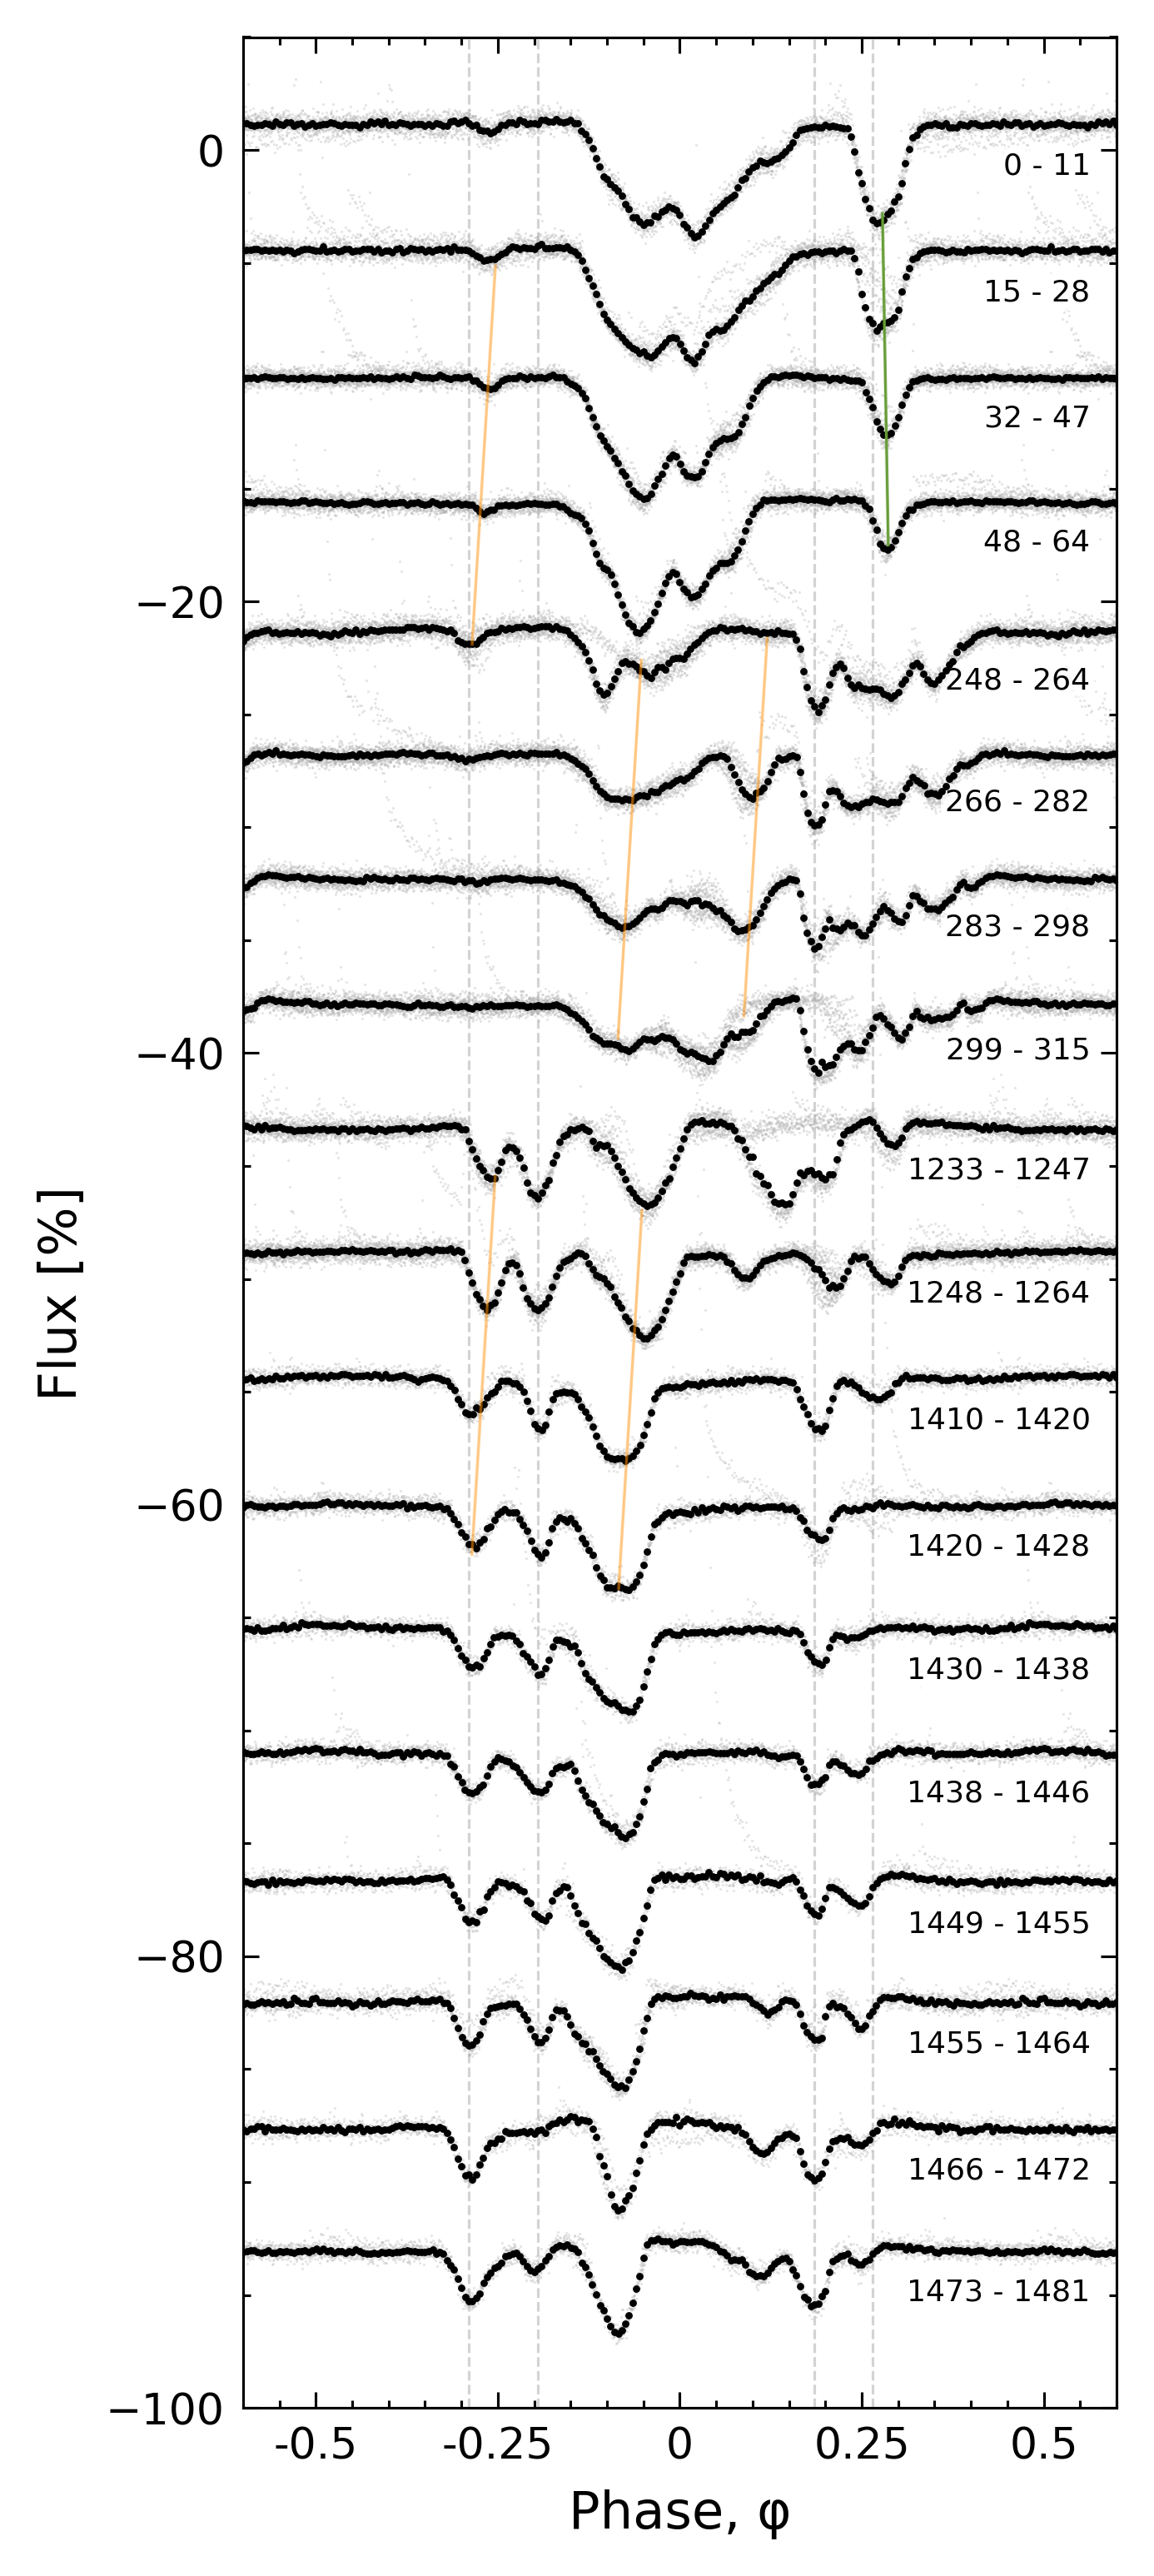
\includegraphics[width=0.45\textwidth]{ANNOTATED_resid_TIC_402980664_P18.5611_2min_phase_timegroups.png}
    	\end{center}
    \vspace{-0.4cm}
		\caption{
	      {\bf Alternative view of the evolution of LP 12-502}
	      (Figure~\ref{fig:lp}), arranged to emphasize changes in transit
	      times.  There are 200 binned black points per cycle; a two-harmonic
	      sinusoid has been subtracted over specific chunks in time ({\bf see text}).
	      Vertical gray lines are underplotted to help guide the eye to instances
	      in which preferred dip phases synchronize over long baselines.
	      The orange and green lines guide the eye to where dips
	      appear to change the positions of their local minima.
		}
		\label{fig:lp2}
\end{figure*}


\begin{figure*}[!t]
	\begin{center}
		\subfloat{
			\includegraphics[width=0.43\textwidth]{TIC402980664_river_gist_stern_0_64_manual_20230617_mask_v0_nterms2_vmin-0.04000_vmax0.01000.png}
			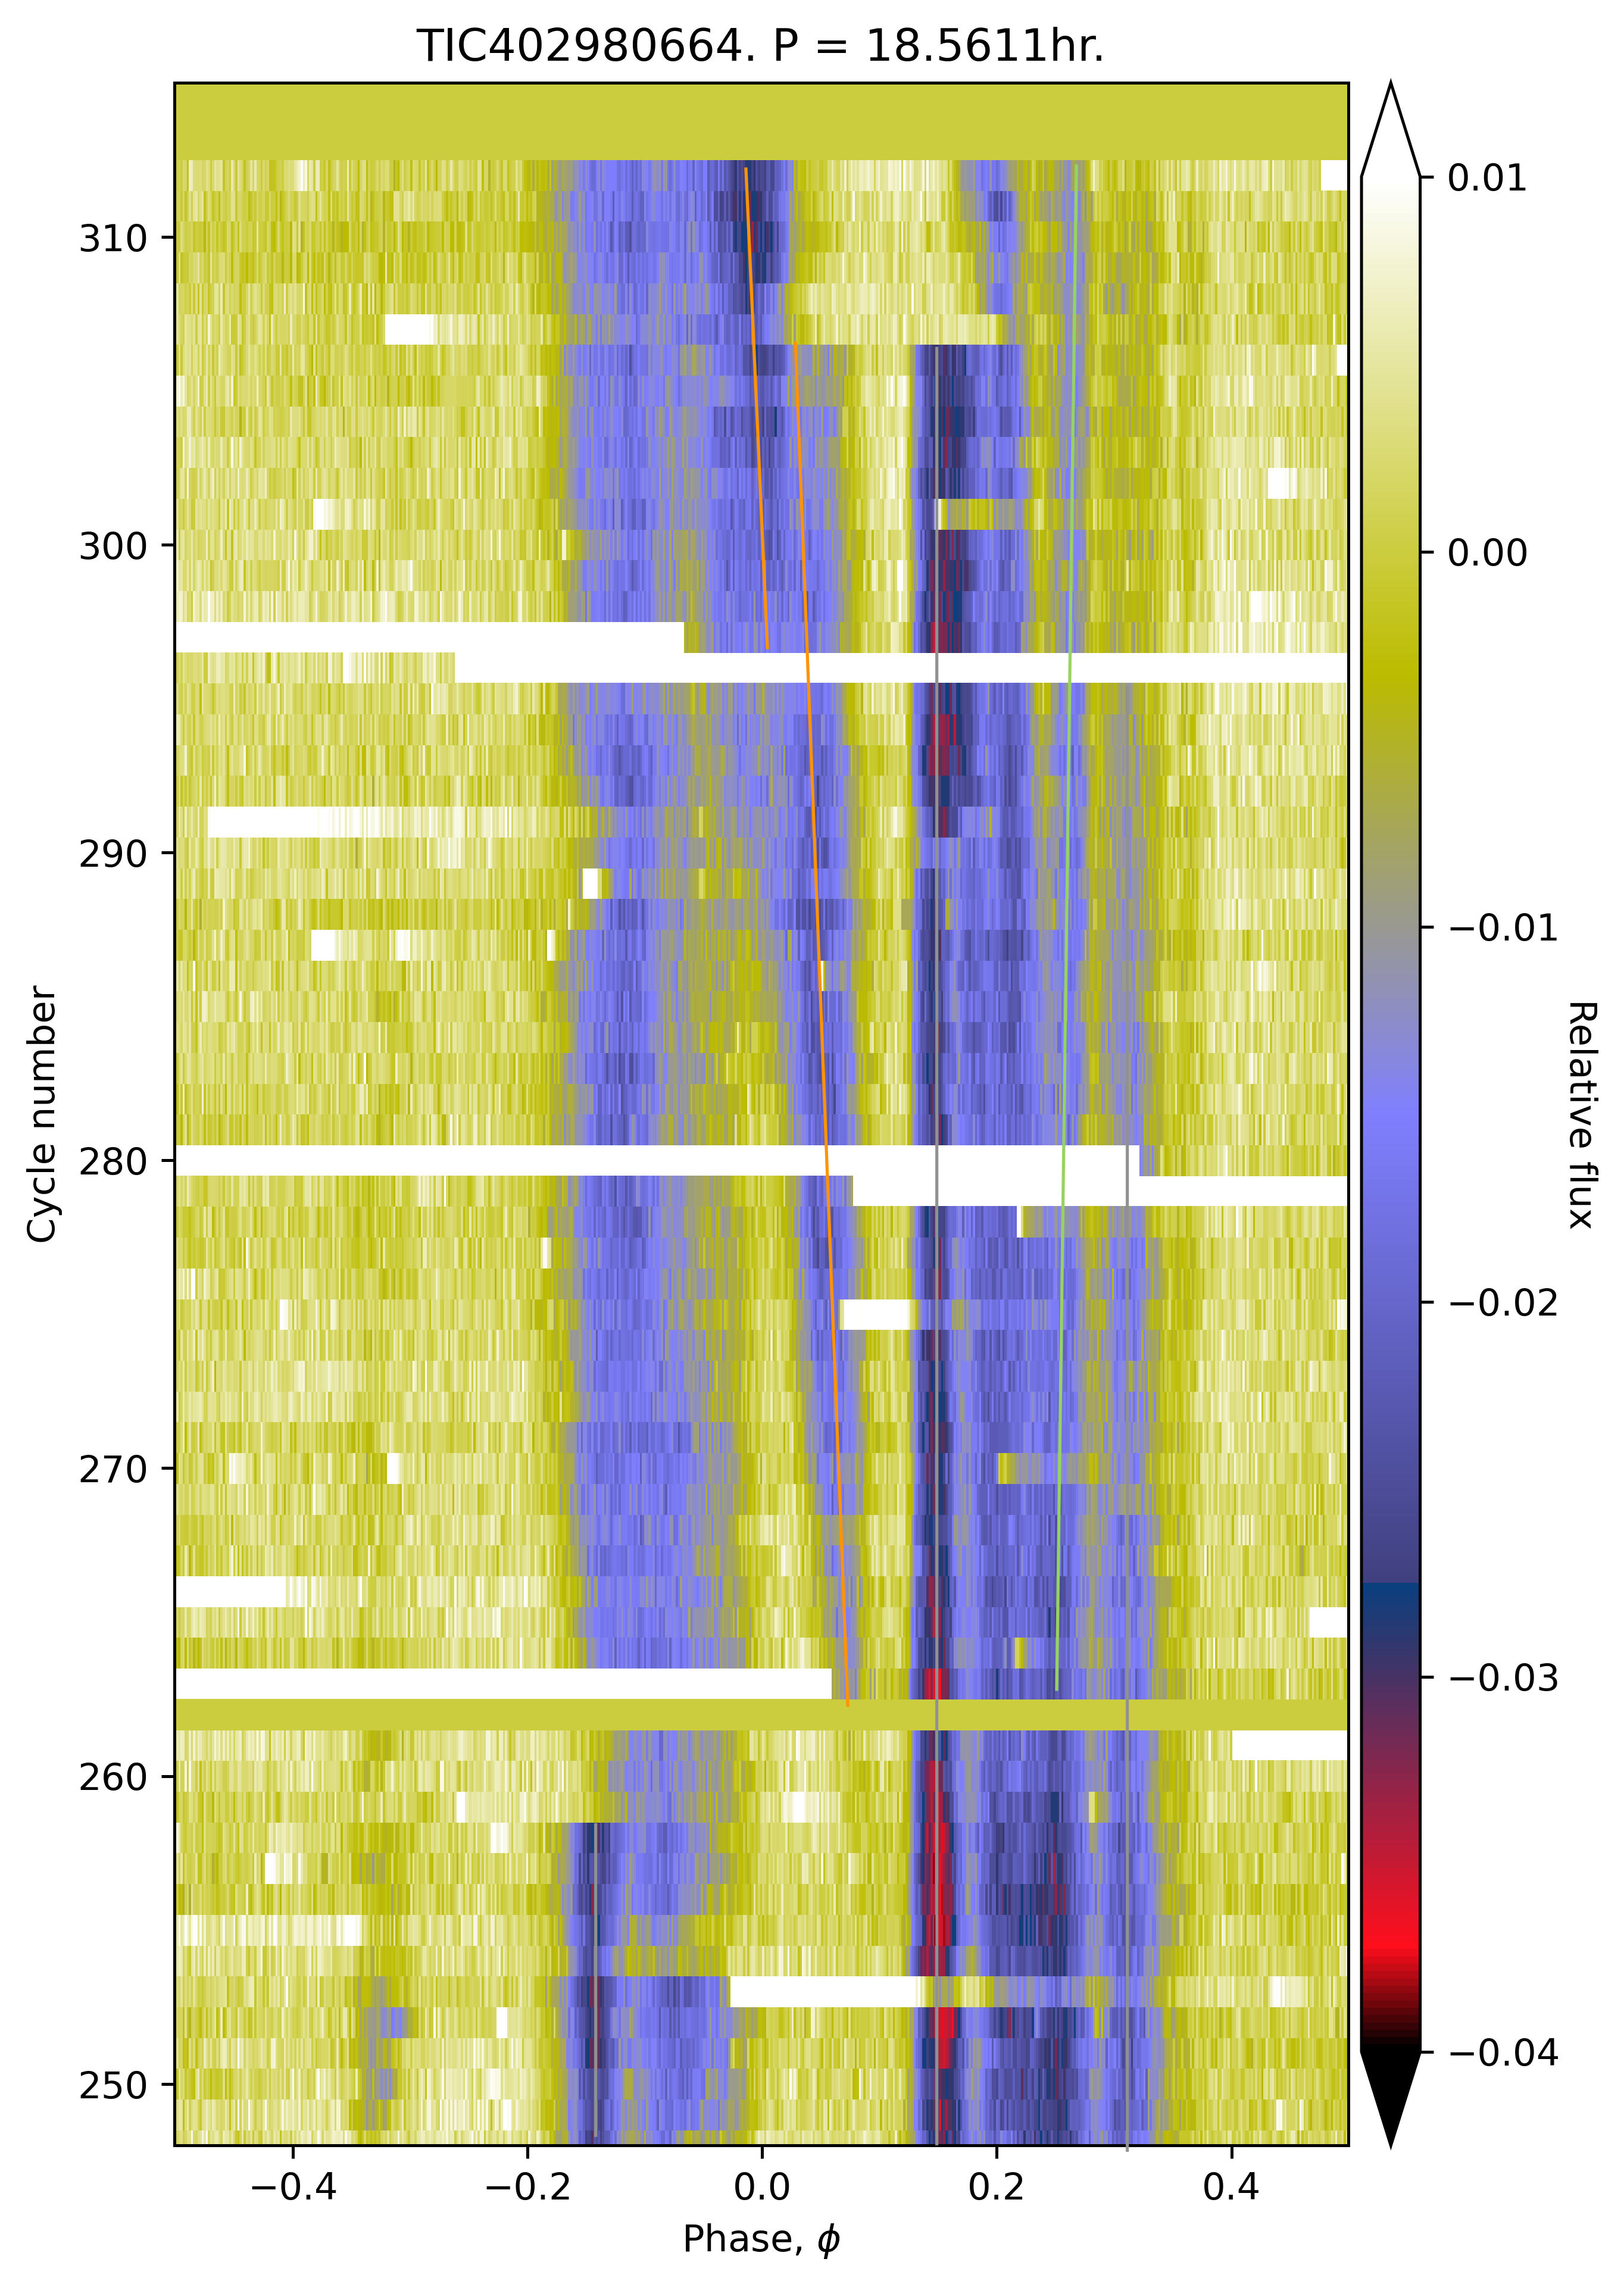
\includegraphics[width=0.43\textwidth]{ANNOTATED_TIC402980664_river_gist_stern_248_315_manual_20230617_mask_v0_nterms2_vmin-0.04000_vmax0.01000.png}
		}
	\vspace{-1cm}
			\subfloat{
		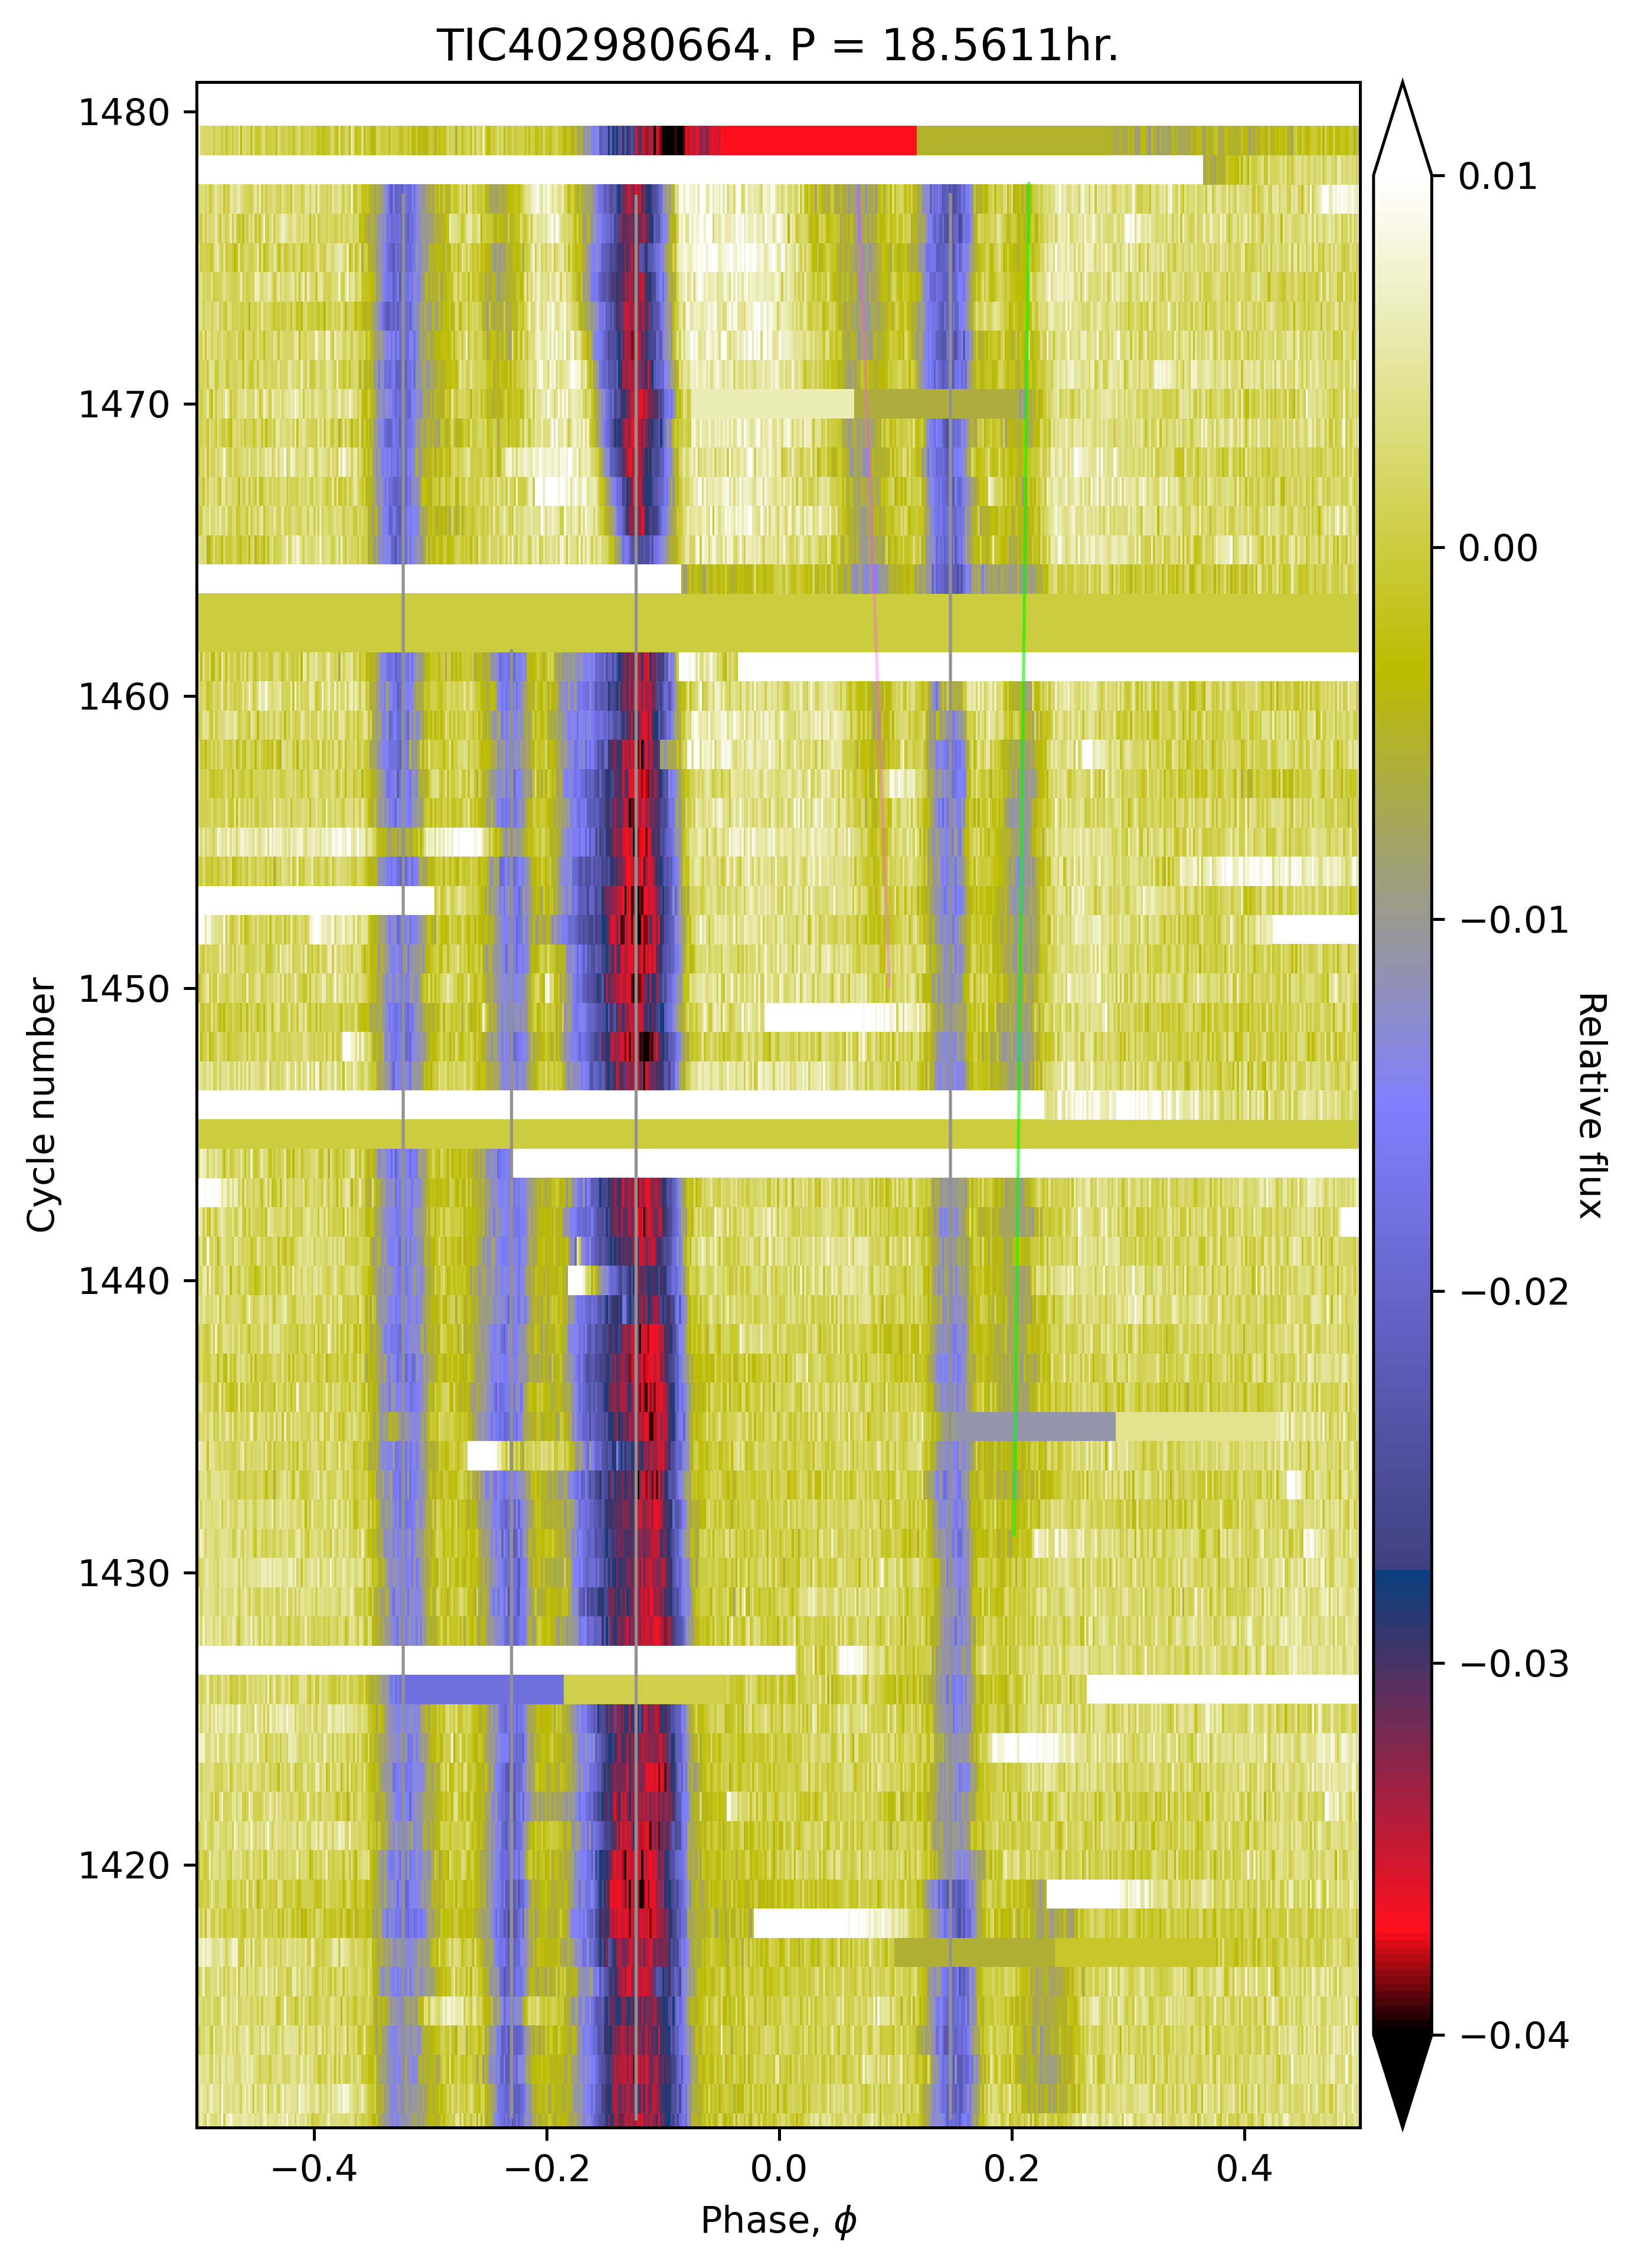
\includegraphics[width=0.43\textwidth]{ANNOTATED_TIC402980664_river_gist_stern_1411_1481_manual_20230617_mask_v0_nterms2_vmin-0.04000_vmax0.01000.png}
				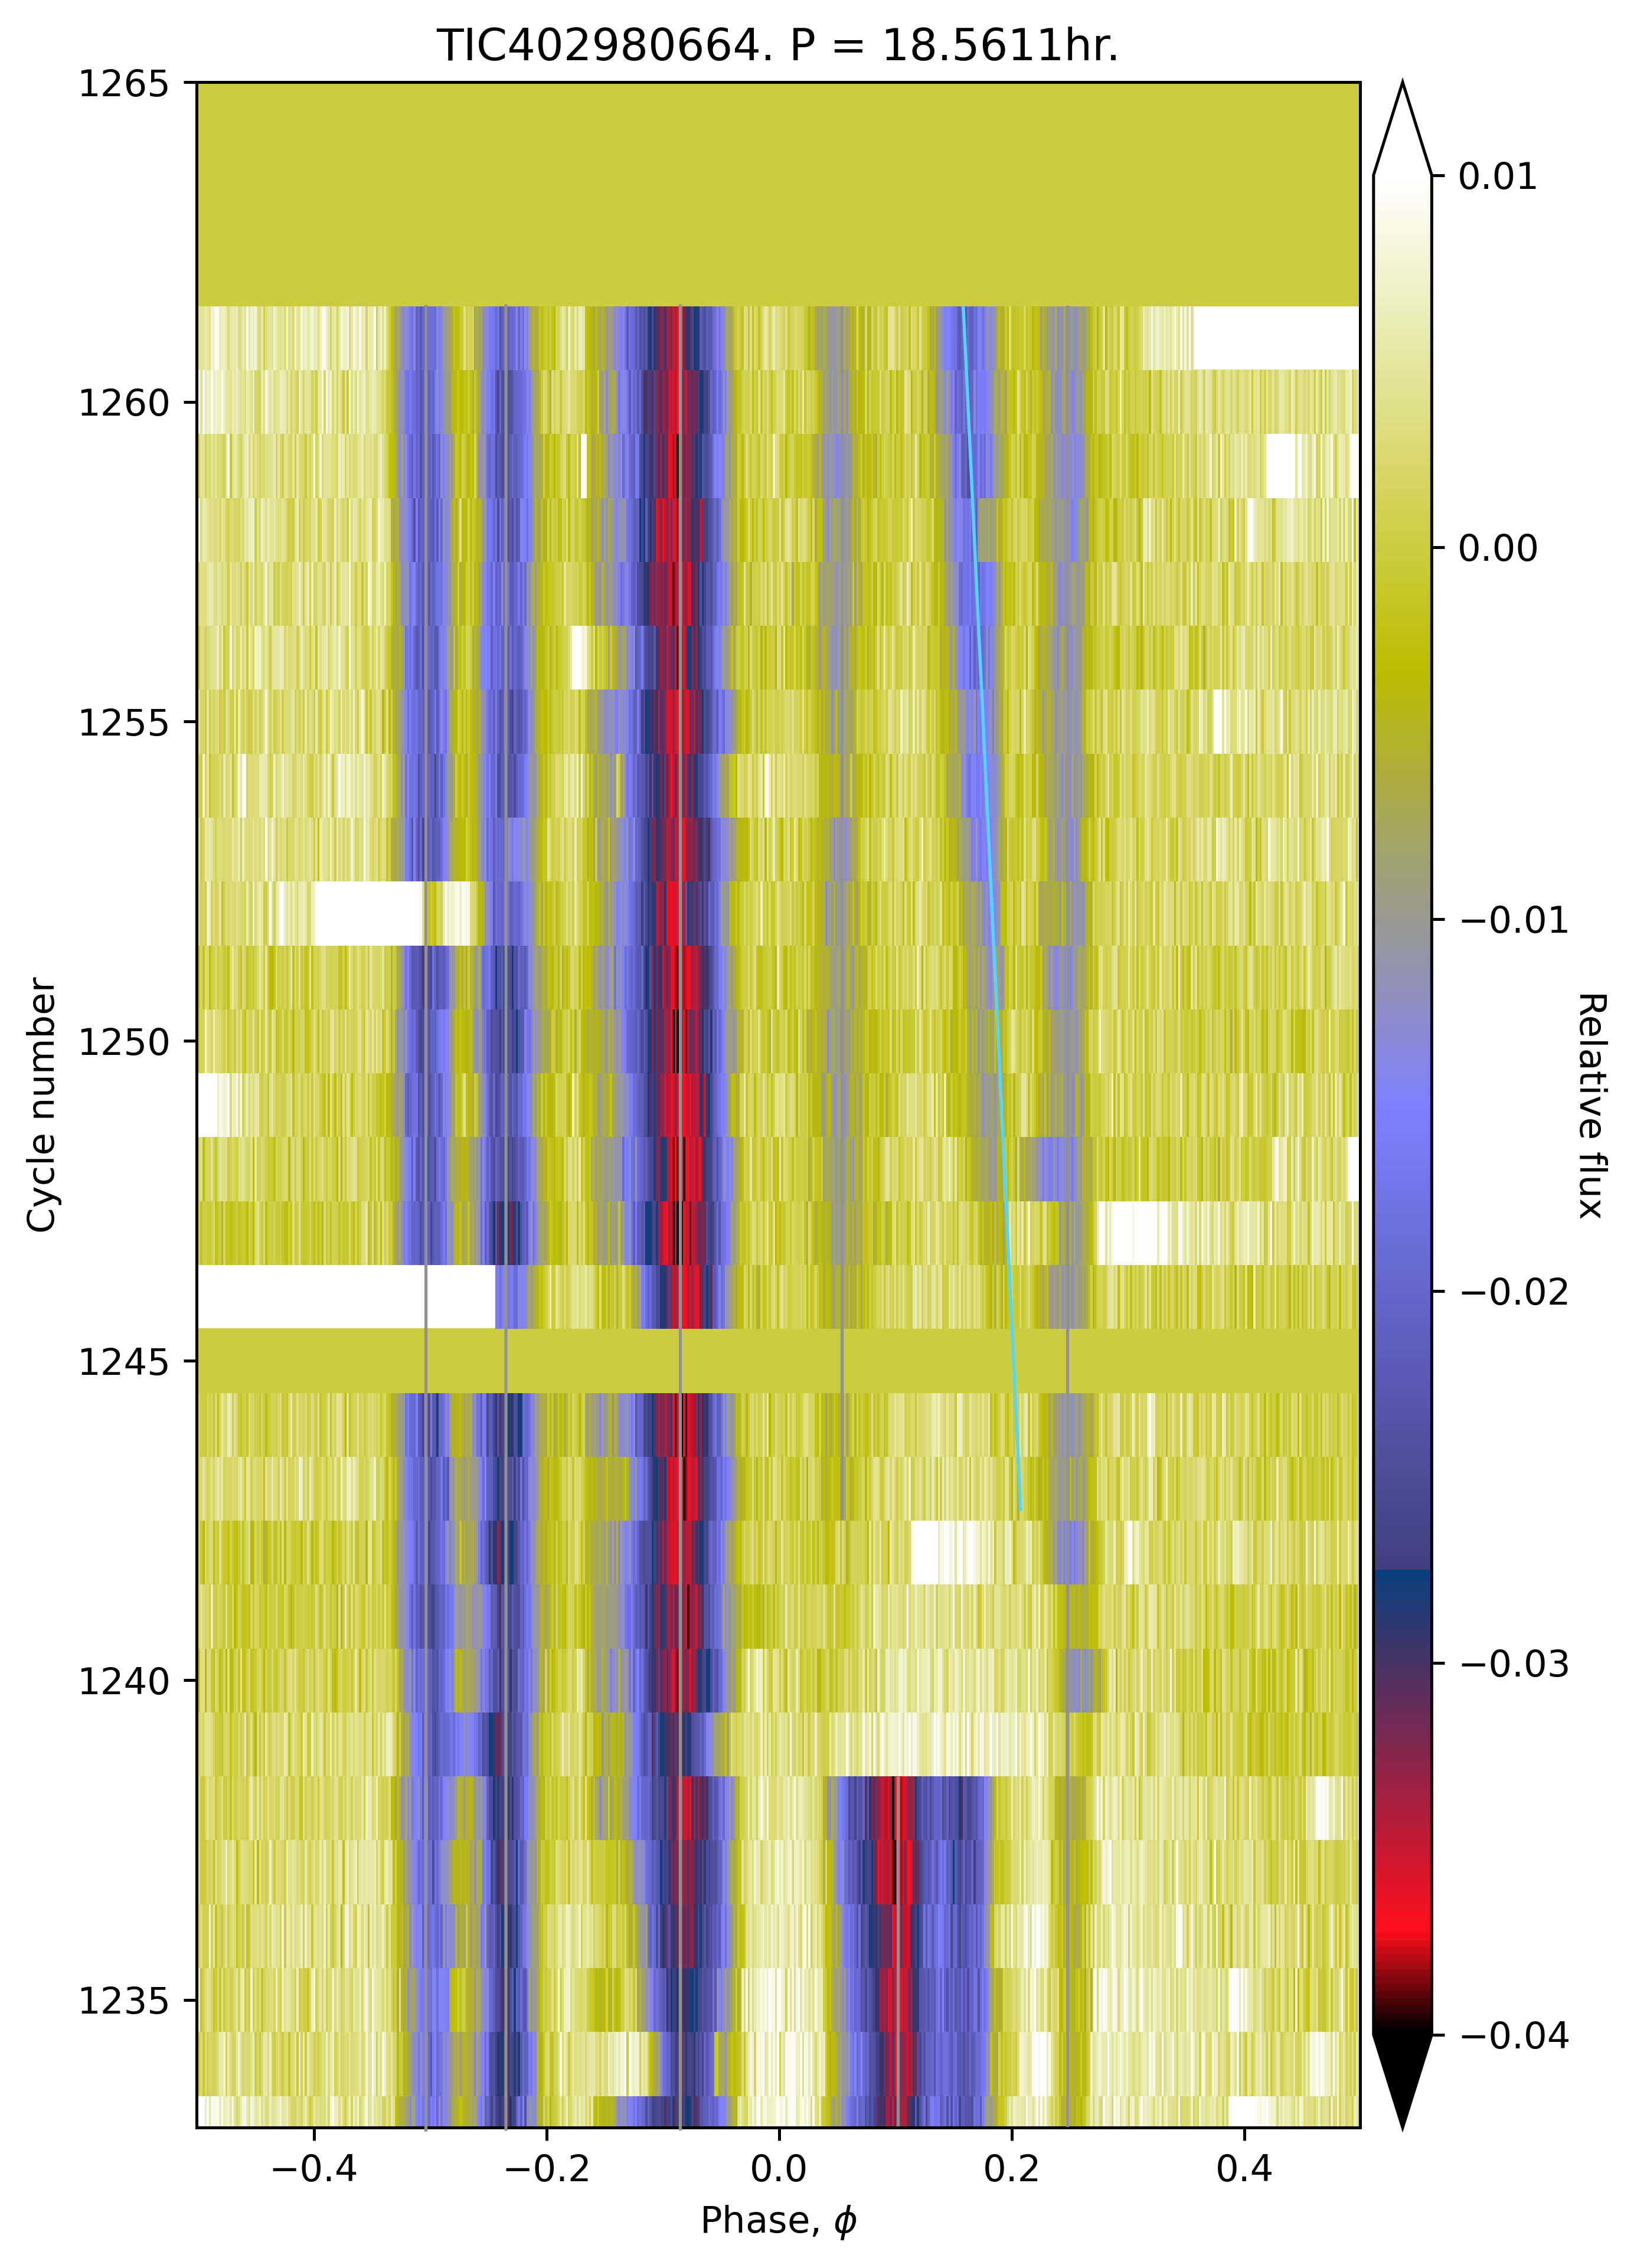
\includegraphics[width=0.43\textwidth]{ANNOTATED_TIC402980664_river_gist_stern_1233_1265_manual_20230617_mask_v0_nterms2_vmin-0.04000_vmax0.01000.png}
	}
	\end{center}
	\vspace{-0.4cm}
	\caption{
    {\bf River plots of LP 12-502}, showing (clockwise from top-left)
    Sectors 18-19, 25-26, 53, and 58-59.  A two-harmonic sinusoid has
    been subtracted over specific chunks in time ({\bf see text}).
    For Sectors 25-26 (cycles 248-315), three periods are overplotted:
    $P$=18.5611\,hr (gray vertical line); 18.5404\,hr (orange); 18.5683\,hr (green).
    For Sector 53, gray is identical, while cyan is 18.5145\,hr.
    For Sectors 58-59, the magenta line is 18.5473\,hr, and the green
    line is 18.5672\,hr.
	}
	\label{fig:lpriver0}
\end{figure*}

\section{More river plots}

Figures~\ref{fig:tic3006river} and~\ref{fig:tic3006timegroups} show 120-second
cadence data for TIC~300651846, a CQV in the TESS continuous viewing zone.
With the exception of a few sectors, TESS data will exist for this source
over Sectors 1-12, 27-39, and 61-69.
The majority are in the full frame images, and are the subject of future work.

\begin{figure*}[!t]
	\begin{center}
		\subfloat{
			\includegraphics[width=0.43\textwidth]{TIC300651846_river_seismic_0_650_vmin-0.06000_vmax0.06000.png}
			\includegraphics[width=0.43\textwidth]{TIC300651846_river_seismic_2305_2630_vmin-0.06000_vmax0.06000.png}
		}
	\end{center}
	\vspace{-0.4cm}
	\caption{
		{\bf River plots of TIC 300651846}.
		The envelope has not been subtracted.
		7 sectors of continuous 2-minute observations S32-S39.  (Thanks to DDT029)
		Then a few in S60+ on the right.
		Compare to Figure~\ref{fig:cqvs}.
	}
	\label{fig:tic3006river}
\end{figure*}

\begin{figure*}[!t]
	\begin{center}
		\subfloat{
			\includegraphics[width=0.43\textwidth]{TIC_300651846_P8.254_2min_phase_timegroups.png}
		}
	\end{center}
	\vspace{-0.4cm}
	\caption{
		{\bf Orbit-phased plots of TIC 300651846}.
		The envelope has not been subtracted.
	}
	\label{fig:tic3006timegroups}
\end{figure*}


\section{No significant power at 20~second cadence}

TESS was the first instrument to show that CQV light curves contain
power at timescales of a few minutes
\citep{127Z,2020AJ....160...86B,2022AJ....163..144G}.  This advance
was primarily enabled by the fifteen-fold faster cadence in the TESS
2-minute data, relative to K2.

A logical follow-up question to ask is whether the periodic components
of the CQV light curves contain power at timescales below one minute.
Between 2020 and 2021, we observed 10 CQVs at 20-second cadence with
TESS in order to explore this question (TESS DDT029).  The stars were
TICs 142173958, 146539195, 24518895, 276453848, 264599508, 363963079,
144486786, 408188366, 300651846, 262400835.  The general conclusion
derived from comparing the 20-second to 120-second data for these
stars (available on MAST) was that CQVs do not contain appreciable
power at this timescale.

% \section{Chromaticity in TIC 262400835}
% 
% TIC~262400835 ($d$=174\,pc) is formally outside the scope of the
% current work.  However, this CQV was observed using MuSCAT2 on 2020
% December 12, 13, and 16, and the results might be worth including in
% this study.
% {\bf todo: describe observations / decide whether to include!}.
% 
% We include {\bf a table of the photometry} here to enable potential
% future deeper analyses of the chromaticity of this object class.
% 
% Generally, these data serve as a minor addition beyond the
% observations that have been acquired by
% \citet[e.g.][]{2017PASJ...69L...2O,2020PASJ...72...23T,2022AJ....163..144G,2023MNRAS.518.2921K}
% on this topic.  \citet{2023MNRAS.518.2921K} provides what we find to
% be the most lucid summary, and we quote: ``amplitudes are almost
% always larger, the shorter the wavelength of the filter, but the
% relationship can be weak or non-monotonic.''
% 
% \begin{figure*}[!t]
% 	\begin{center}
%     \includegraphics[width=0.45\textwidth]{TIC262400835_multicolor_phase_stacked.pdf}
%     	\end{center}
%     \vspace{-0.4cm}
% 		\caption{
% 	      {\bf Chromaticity in TIC~262400835}.
% 		}
% 		\label{fig:muscat}
% \end{figure*}



\clearpage
\listofchanges


\end{document}
